\documentclass[10pt,a4paper]{article}
\usepackage[T1]{fontenc}
\usepackage{lmodern,amsmath,amssymb,booktabs,array,xcolor,microtype}
\usepackage[margin=16mm,top=14mm,bottom=16mm]{geometry}
\usepackage{fancyhdr,tikz,graphicx}
\usepackage[hidelinks]{hyperref}
\definecolor{navy}{HTML}{17394D}
\definecolor{teal}{HTML}{176E78}
\definecolor{pale}{HTML}{EEF5F7}
\definecolor{muted}{HTML}{4B5963}
\definecolor{rulegray}{HTML}{CAD5DB}
\setlength{\parindent}{0pt}
\setlength{\parskip}{3pt}
\setlength{\abovedisplayskip}{4pt}
\setlength{\belowdisplayskip}{4pt}
\setlength{\abovedisplayshortskip}{3pt}
\setlength{\belowdisplayshortskip}{3pt}
\pagestyle{fancy}\fancyhf{}
\renewcommand{\headrulewidth}{0pt}
\fancyfoot[L]{\scriptsize\color{muted}QVDF-E \quad | \quad Emission calculation reference}
\fancyfoot[R]{\scriptsize\color{muted}\thepage\ / 6}
\newcommand{\method}[2]{\par\vspace{4pt}{\color{teal}\bfseries #1\quad #2}\par\vspace{1pt}}
\newcommand{\notebox}[1]{\par\vspace{4pt}\begingroup\setlength{\fboxsep}{7pt}\colorbox{pale}{\parbox{\dimexpr\linewidth-14pt\relax}{#1}}\endgroup\par}
\hypersetup{pdftitle={QVDF-E: Five emission calculations and evaluation results},pdfauthor={Mohammad Abbasi},pdfsubject={Equations and verified average-weekday results}}
\definecolor{methodO}{HTML}{242B33}
\definecolor{methodS}{HTML}{0072B2}
\definecolor{methodR}{HTML}{7B3294}
\definecolor{methodM}{HTML}{009E73}
\definecolor{methodA}{HTML}{D55E00}\newcommand{\legendkey}[2]{{\scriptsize\textcolor{#1}{\rule[2pt]{10pt}{1.3pt}}\ #2}}
\begin{document}
\fontsize{9.3}{11.1}\selectfont
{\fontsize{19}{22}\selectfont\bfseries\color{navy}Five emission calculations}\par
{\color{muted}One whole episode, one pollutant. O, S, R, M and A identify the existing calculations.}

\textbf{Notation and units.} Bin $i$ has speed $v_i$ and count $d_i=q_i\Delta t$, with $\Delta t=1/12$ h.
$D=\sum_i d_i$; $L$ is link length; $C$ is hourly capacity; $T_f=L/v_f$.
$H$ denotes vehicle-hours, $P$ episode duration and $T$ per-vehicle travel time.
$r_0(v)$ is the zero-acceleration lookup rate in g/(veh\,h); $E$ is in grams. Counts and capacity use the same lane basis.

\textbf{Shared fitted quantities for R, M and A.}
\[
x=\frac{D}{C},\qquad \widehat P=\max(f_dx^n,x),\qquad
\widehat w_{\max}=T_f f_p\widehat P^{s},\qquad
\widehat{\bar w}=\theta\widehat w_{\max},\qquad
H_{\rm pred}=D(T_f+\widehat{\bar w}).
\]
$f_d,n,f_p,s,\theta$ are calibrated by directional corridor and period, with the existing sparse-period fallback.

\method{O}{Recorded-speed reference}
Assign each bin's counted vehicles the complete-link travel time $L/v_i$, then sum:
\[
H_i=d_i\frac{L}{v_i},\qquad H_{\rm obs}=\sum_i H_i,\qquad
\boxed{E_O=\sum_i H_i r_0(v_i).}
\]
The five-minute interval supplies the count; emission exposure is $L/v_i$, not five minutes.

\method{S}{Episode mean-speed estimate}
Use the count-weighted harmonic mean, preserving the reference's total vehicle-hours:
\[
\bar v_{\rm obs}=\frac{D}{\sum_i d_i/v_i}=\frac{DL}{H_{\rm obs}},\qquad
\boxed{E_S=H_{\rm obs}\,r_0(\bar v_{\rm obs}).}
\]

\method{R}{Reconstructed whole-link speeds}
For normalized entry time $u\in[0,1]$, define $w(u)=\widehat w_{\max}h(u)$ and
$v_R(u)=L/[T_f+w(u)]$. The symmetric profile is
\[
h(u)=\begin{cases}
[4u(1-u)]^a,&\theta\le 2/3,\quad \int_0^1h(u)\,du=\theta\ \text{determines }a,\\
1-|2u-1|^b,&\theta>2/3,\quad b=\theta/(1-\theta).
\end{cases}
\]
The entering-vehicle weight is $dN=D[1+(\widehat w_{\max}/\widehat P)h'(u)]\,du$. Thus
\[
\boxed{E_R=\int_0^1[T_f+w(u)]\,r_0\!\left(\frac{L}{T_f+w(u)}\right)\,dN.}
\]
The integral uses 384 quadrature points; $\int dN=D$ and $\int[T_f+w(u)]dN=H_{\rm pred}$.
These are trip-average speeds by entry time, not individual operating-speed trajectories.

\method{M}{Two-speed lookup}
Infer the queue speed from discharge and the triangular fundamental diagram:
\[
\widehat\mu=\frac{D}{\widehat P},\qquad
\omega=\frac{C}{k_j-C/v_f},\qquad
\widehat v_q=\frac{\widehat\mu}{k_j-\widehat\mu/\omega},\qquad k_j=220\ \text{veh/mi/lane}.
\]
Allocate mean travel time between two operating speeds while preserving distance:
\[
\bar T_q=\frac{v_f\widehat{\bar w}}{v_f-\widehat v_q},\qquad
\bar T_{\rm free}=T_f-\frac{\widehat v_q\widehat{\bar w}}{v_f-\widehat v_q},\qquad
\boxed{E_M=D[\bar T_{\rm free}r_0(v_f)+\bar T_qr_0(\widehat v_q)].}
\]
Here $\bar T_{\rm free}+\bar T_q=T_f+\widehat{\bar w}$ and $v_f\bar T_{\rm free}+\widehat v_q\bar T_q=L$.

\method{A}{Two-speed cubic}
Keep M's speeds and times; replace the lookup rate by its fitted cubic:
\[
r_c(v)=c_0+c_1v+c_2v^2+c_3v^3,\qquad
\boxed{E_A=D[\bar T_{\rm free}r_c(v_f)+\bar T_qr_c(\widehat v_q)].}
\]

\notebox{\textbf{Evaluation: episode-total WAPE.} For method $m\in\{S,R,M,A\}$ and the same $N=137$ episodes,
\[
\boxed{\operatorname{WAPE}_m=100\frac{\sum_{k=1}^{N}|E_{m,k}-E_{O,k}|}{\sum_{k=1}^{N}E_{O,k}}.}
\]
Absolute errors are calculated before pooling episodes. O is a detector-speed-based calculation,
not measured emissions or observed vehicle trajectories. All five calculations omit acceleration effects.}

\newpage
\fontsize{10}{12.4}\selectfont
{\fontsize{19}{22}\selectfont\bfseries\color{navy}Results on the common episode sample}\par
{\color{muted}137 average-weekday episodes: 20 Arizona I-10 and 117 California PeMS.}\par
\vspace{8pt}
\textbf{Table 1. CO$_2$ totals, travel-time exposure and episode-total error.}

\renewcommand{\arraystretch}{1.65}
\setlength{\tabcolsep}{5pt}
\begin{tabular*}{\linewidth}{@{\extracolsep{\fill}}lrrrr@{}}
\toprule
\textbf{Calculation} & \shortstack{\textbf{Vehicle-hours}\\\textbf{(veh\,h)}} &
\shortstack{\textbf{Effective rate}\!$^{*}$\\\textbf{kg/(veh\,h)}} &
\shortstack{\textbf{Total CO$_2$}\\\textbf{(kg)}} & \shortstack{\textbf{WAPE}\\\textbf{(\%)}}\\
\midrule
O: recorded speeds & 4,537.48 & 9.063 & 41,123.55 & Reference\\\midrule[0.3pt]
S: episode mean speed & 4,537.48 & 8.646 & 39,231.21 & 5.94\\\midrule[0.3pt]
R: reconstructed speeds & 4,453.44 & 9.623 & 42,856.84 & 10.13\\\midrule[0.3pt]
M: two-speed lookup & 4,453.44 & 11.150 & 49,655.91 & 22.38\\\midrule[0.3pt]
A: two-speed cubic & 4,453.44 & 10.967 & 48,838.84 & 20.32\\
\bottomrule
\end{tabular*}
\par\vspace{3pt}
{\small $^{*}$Effective rate is summed emissions divided by summed vehicle-hours. It is not a lookup rate at a pooled speed. WAPE is based on individual episode errors, not the error of the summed totals.}

\vspace{15pt}
\textbf{Table 2. Episode-total WAPE against O for all four pollutants (\%).}

\begin{tabular*}{\linewidth}{@{\extracolsep{\fill}}lrrrr@{}}
\toprule
\textbf{Calculation} & \textbf{CO$_2$} & \textbf{NO$_x$} & \textbf{CO} & \textbf{HC}\\
\midrule
S: episode mean speed & 5.94 & 12.43 & 6.12 & 4.24\\\midrule[0.3pt]
R: reconstructed speeds & 10.13 & 13.05 & 8.27 & 9.52\\\midrule[0.3pt]
M: two-speed lookup & 22.38 & 47.73 & 11.19 & 12.61\\\midrule[0.3pt]
A: two-speed cubic & 20.32 & 42.71 & 9.82 & 11.65\\
\bottomrule
\end{tabular*}

\vspace{13pt}
\textbf{Reading the comparison}

\textbf{S preserves observed exposure.} It retains O's vehicle-hours and total distance exactly,
changing only how emission rates are averaged. R, M and A use fitted vehicle-hours instead.
The fitted vehicle-hours have an episode WAPE of 14.77\%, although their summed bias is only $-1.85$\%.

\textbf{M versus R isolates a speed-representation difference.} They share the same fitted
vehicle-hours and total distance, but M produces 15.9\% more CO$_2$ and 32.1\% more NO$_x$ in total.
R applies rates to whole-link trip-average speeds; M applies rates to free-flow and queue operating speeds.

\notebox{\textbf{Why one mean speed can be close to the reference}\par
Let $a_i=H_i/H_{\rm obs}$ within an episode. Then $\sum_i a_i=1$ and
$\bar v_{\rm obs}=\sum_i a_iv_i$, giving
\[
E_O-E_S=H_{\rm obs}\left[\sum_i a_i r_0(v_i)-r_0\!\left(\sum_i a_iv_i\right)\right].
\]
If $r_0(v)=a+bv$ over the occupied speed range, S equals O exactly despite speed variability.
The actual stepped lookup is nonlinear, so the discrepancy depends on its rate changes and the speed distribution.}

\vspace{8pt}
\textbf{Interpretation limit.} Lower WAPE means closer agreement with O. It does not establish
greater accuracy against actual vehicle trajectories or measured emissions. A single-speed comparator
using the same fitted exposure, $E_{S,\rm pred}=H_{\rm pred}r_0(DL/H_{\rm pred})$, is not included in these reported results.

\vfill
{\fontsize{8}{10}\selectfont\color{muted}
Source: archived average-weekday episode results and emission metrics (22 September 2026),
filtered to the common five-method sample. Existing outputs were checked and summarized; no experiments were rerun.
Formulas follow the retained implementation. Totals are passenger-car-equivalent estimates on the source per-lane basis.}
% DETECTOR78_APPENDIX

\newpage
\fontsize{10}{12}\selectfont
{\fontsize{19}{22}\selectfont\bfseries\color{navy}Detector 78: worked link example}\par
{\color{muted}Arizona I-10 westbound, January 2016 average weekday.}

\notebox{\textbf{Scope.} This is the standalone workbook example from the supplied sensor-78 data:
16 complete weekdays, 57 bins from 14:45 inclusive to 19:30 exclusive. The window is fixed for explanation,
not newly detected. These inputs differ from the archived paper sample; the case is not one of the
137 observations summarized on page 2. Supplied counts are assumed already per lane (multiplier 1).}

\vspace{7pt}\textbf{Inputs and fitted traffic quantities}\par
\renewcommand{\arraystretch}{1.35}\setlength{\tabcolsep}{6pt}
\begin{tabular*}{\linewidth}{@{\extracolsep{\fill}}lrlr@{}}\toprule
Input & Value & Calculated quantity & Value\\\midrule
Link length $L$ & 1.040 mi & Demand $D$ & 4,789.25 veh/lane\\
Free-flow speed $v_f$ & 64.161 mph & $D/C$ & 3.189 h\\
Capacity $C$ & 1,501.616 veh/h/lane & Predicted duration $\widehat P$ & 4.449 h\\
Jam density $k_j$ & 220 veh/mi/lane & Queue speed $\widehat v_q$ & 13.611 mph\\
Observed duration & 4.750 h & Predicted mean delay & 1.496 min\\
Observed vehicle-hours & 211.434 veh h/lane & Predicted vehicle-hours & 197.040 veh h/lane\\
Observed mean speed & 23.557 mph & Predicted mean trip speed & 25.278 mph\\\bottomrule
\end{tabular*}
\par\smallskip
{\small Calibration: $f_d=1.693177$, $n=0.833031$, $f_p=0.308070$, $s=1.635098$, $\theta=0.434829$ (PM).
The reconstructed shape exponent is $a=3.396386$.}

\vspace{9pt}\textbf{How the CO$_2$ totals are obtained}
\begin{align*}
E_O &= \sum_{i=1}^{57}d_i(L/v_i)r_0(v_i)/1000 = 1,743.79\ \text{kg/lane},\\
E_S &= 211.434\times 6,931.846 /1000 = 1,465.63\ \text{kg/lane},\\
E_R &= \sum_{j=1}^{384}N_j[T_f+w(u_j)]r_0(v_R(u_j))/1000
      = 1,657.64\ \text{kg/lane},\\
E_M &= 4,789.25[0.00949555\times 20,615.635+0.03164658\times 6,931.846]/1000
      = 1,988.14\ \text{kg/lane},\\
E_A &= 4,789.25[0.00949555\times 18,172.460+0.03164658\times 6,680.499]/1000
      = 1,838.94\ \text{kg/lane}.
\end{align*}
The numerical rates are in g/(veh h), times in hours; dividing by 1,000 converts grams to kg.
For O the displayed result is converted to kg after summation. For R, $N_j$ are quadrature vehicle weights.
Unrounded values are used in the calculations; the substitutions above are rounded.

\notebox{\textbf{The speed/rate distinction in this case.}
The observed mean speed is 23.557 mph and the inferred queue speed is 13.611 mph;
both select the same CO$_2$ lookup rate, 6,931.846 g/(veh h).
Free-flow speed selects 20,615.635 g/(veh h).
M assigns 23.1\% of its vehicle-hours to free flow, which contributes 47.2\% of its CO$_2$ total.
Its mean trip consists of 0.570 min at free flow and 1.899 min at queue speed.}

\vspace{8pt}\textbf{Episode emission totals and CO$_2$ discrepancy}\par
\renewcommand{\arraystretch}{1.4}\setlength{\tabcolsep}{4pt}
\begin{tabular*}{\linewidth}{@{\extracolsep{\fill}}lrrrrr@{}}\toprule
Calculation & CO$_2$ (kg) & NO$_x$ (g) & CO (g) & HC (g) & CO$_2$ error (\%)\\\midrule
O: Recorded speeds & 1,743.79 & 1,400.82 & 15,511.48 & 658.66 & Reference \\
S: Episode mean speed & 1,465.63 & 861.78 & 13,252.81 & 581.74 & -15.95 \\
R: Reconstructed speeds & 1,657.64 & 1,360.90 & 14,045.02 & 609.22 & -4.94 \\
M: Two-speed lookup & 1,988.14 & 1,997.71 & 15,645.69 & 665.78 & +14.01 \\
A: Two-speed cubic & 1,838.94 & 1,712.13 & 14,960.73 & 641.44 & +5.46 \\
\bottomrule\end{tabular*}
\par\smallskip{\small Totals are per lane. Signed error is $100(E_m/E_O-1)$;
its absolute value is the one-episode WAPE. R has the smallest CO$_2$ discrepancy here.
M's absolute discrepancy (14.01\%) is smaller than S's (15.95\%), unlike the pooled ordering on page 2.}
\vfill
{\small\color{muted}Source: Sensor78\_Emission\_Calculations.xlsx and its embedded January input profile and calibrated parameters.
Recorded source travel times are not used: link times are recalculated as $L/v$. All emissions use passenger-car rates with zero acceleration and level road.}


\newpage
{\fontsize{18}{21}\selectfont\bfseries\color{navy}All five methods on the same clock}\par
{\color{muted}Detector 78. The modeled groups are aligned to the recorded cumulative vehicle counts.}\par
\legendkey{methodO}{O: recorded}\quad\legendkey{methodS}{S: mean speed}\quad\legendkey{methodR}{R: reconstructed}\quad\legendkey{methodM}{M: two-speed}\quad\legendkey{methodA}{A: cubic}
\begin{center}\resizebox{\linewidth}{!}{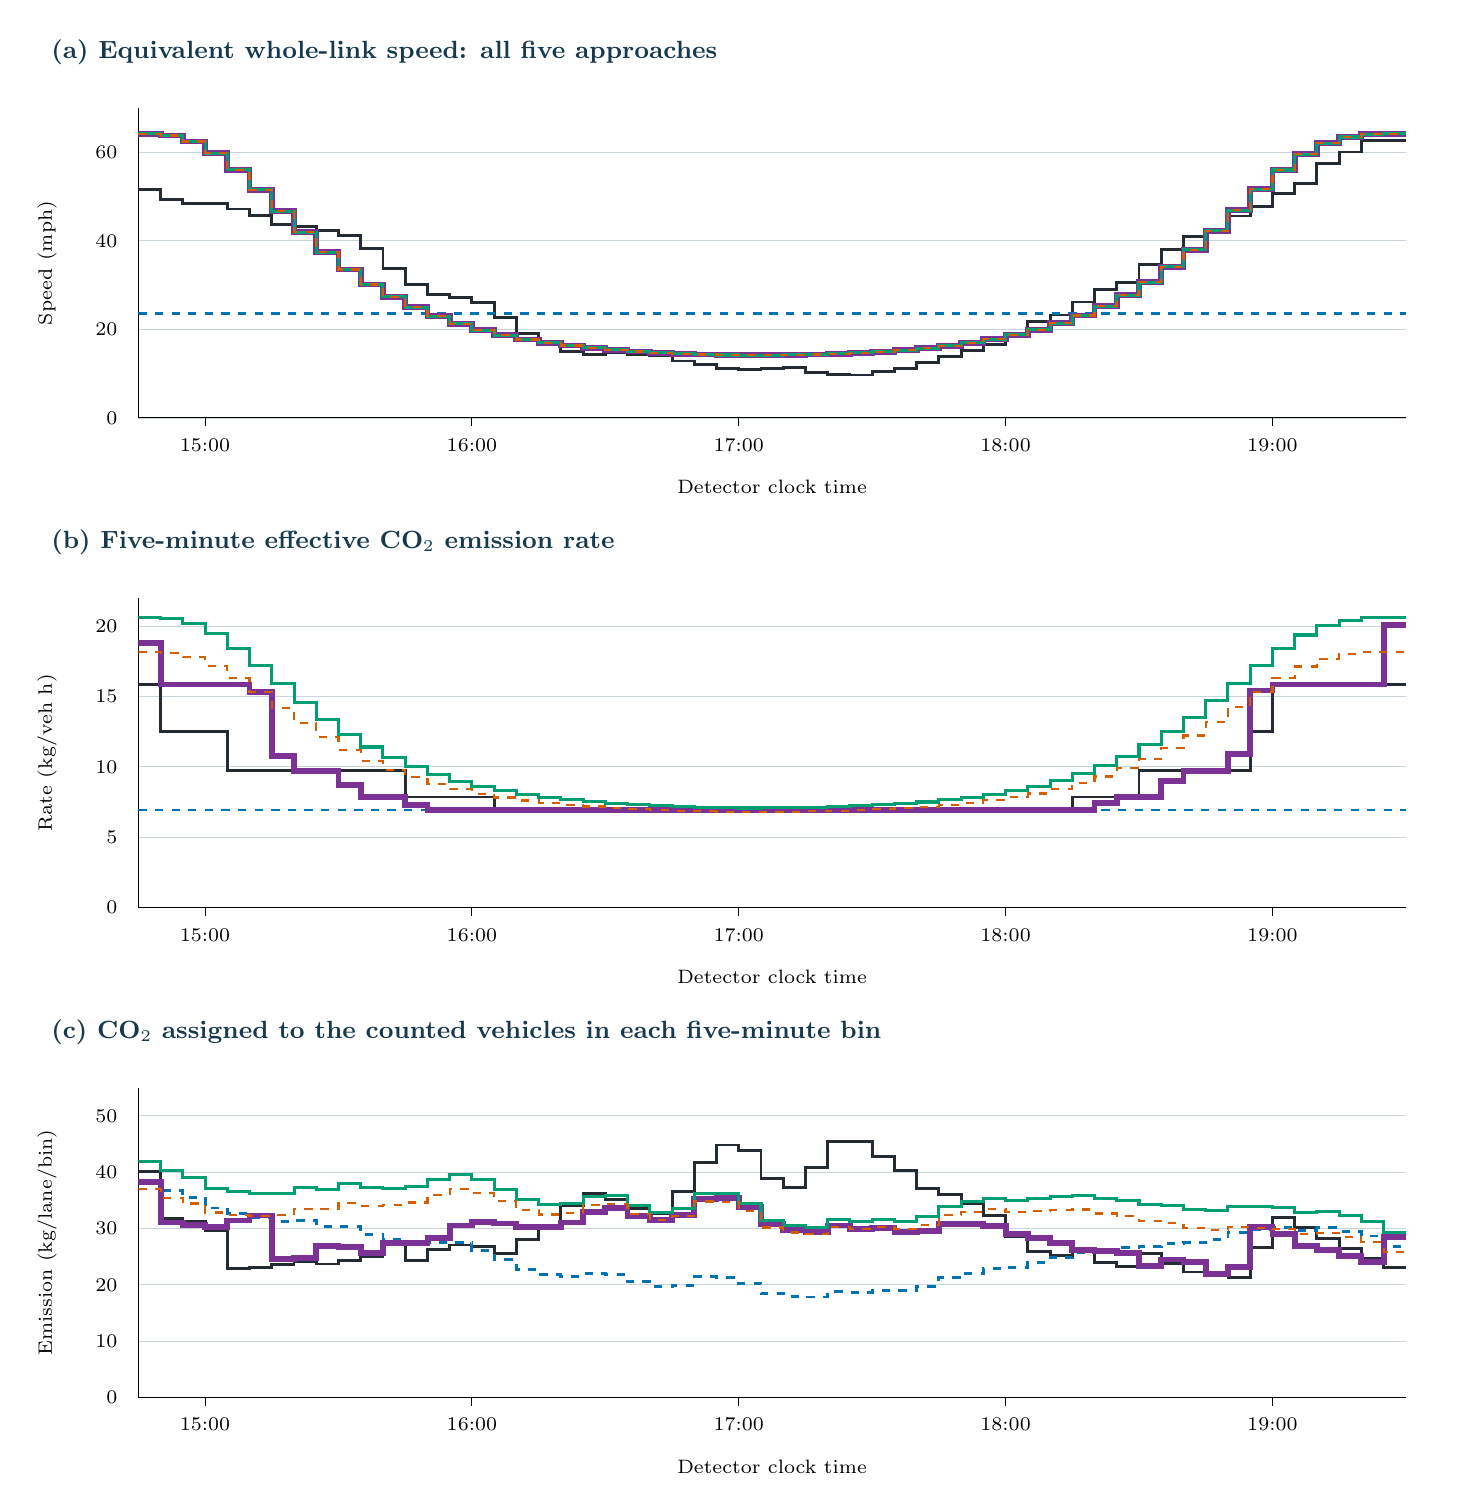
\begin{tikzpicture}[x=1pt,y=1pt]
\useasboundingbox (0,0) rectangle (509,524);
\node[anchor=west,font=\small\bfseries,text=navy] at (5,515) {(a) Equivalent whole-link speed: all five approaches};
\draw[rulegray,line width=.25pt] (40,383.000) -- (498,383.000);
\node[anchor=east,font=\scriptsize] at (36,383.000) {0};
\draw[rulegray,line width=.25pt] (40,415.000) -- (498,415.000);
\node[anchor=east,font=\scriptsize] at (36,415.000) {20};
\draw[rulegray,line width=.25pt] (40,447.000) -- (498,447.000);
\node[anchor=east,font=\scriptsize] at (36,447.000) {40};
\draw[rulegray,line width=.25pt] (40,479.000) -- (498,479.000);
\node[anchor=east,font=\scriptsize] at (36,479.000) {60};
\draw[black,line width=.35pt] (64.105,383) -- (64.105,380);
\node[anchor=north,font=\scriptsize] at (64.105,379) {15:00};
\draw[black,line width=.35pt] (160.526,383) -- (160.526,380);
\node[anchor=north,font=\scriptsize] at (160.526,379) {16:00};
\draw[black,line width=.35pt] (256.947,383) -- (256.947,380);
\node[anchor=north,font=\scriptsize] at (256.947,379) {17:00};
\draw[black,line width=.35pt] (353.368,383) -- (353.368,380);
\node[anchor=north,font=\scriptsize] at (353.368,379) {18:00};
\draw[black,line width=.35pt] (449.789,383) -- (449.789,380);
\node[anchor=north,font=\scriptsize] at (449.789,379) {19:00};
\draw[black,line width=.45pt] (40,495) -- (40,383) -- (498,383);
\node[anchor=north,font=\scriptsize] at (269.0,364) {Detector clock time};
\node[rotate=90,font=\scriptsize] at (7,439.0) {Speed (mph)};
\begin{scope}
\clip (40,383) rectangle (498,495);
\draw[methodO,line width=1.05pt,] plot coordinates {(40.000,465.599) (48.035,465.599) (48.035,461.879) (56.070,461.879) (56.070,460.542) (64.105,460.542) (64.105,460.571) (72.140,460.571) (72.140,458.461) (80.175,458.461) (80.175,456.225) (88.211,456.225) (88.211,453.002) (96.246,453.002) (96.246,452.181) (104.281,452.181) (104.281,450.852) (112.316,450.852) (112.316,448.982) (120.351,448.982) (120.351,444.291) (128.386,444.291) (128.386,437.101) (136.421,437.101) (136.421,431.084) (144.456,431.084) (144.456,427.713) (152.491,427.713) (152.491,426.390) (160.526,426.390) (160.526,424.596) (168.561,424.596) (168.561,419.119) (176.596,419.119) (176.596,413.500) (184.632,413.500) (184.632,410.175) (192.667,410.175) (192.667,406.865) (200.702,406.865) (200.702,405.975) (208.737,405.975) (208.737,406.496) (216.772,406.496) (216.772,406.031) (224.807,406.031) (224.807,405.687) (232.842,405.687) (232.842,403.551) (240.877,403.551) (240.877,402.351) (248.912,402.351) (248.912,400.911) (256.947,400.911) (256.947,400.410) (264.982,400.410) (264.982,400.951) (273.018,400.951) (273.018,401.201) (281.053,401.201) (281.053,399.442) (289.088,399.442) (289.088,398.542) (297.123,398.542) (297.123,398.490) (305.158,398.490) (305.158,399.810) (313.193,399.810) (313.193,400.820) (321.228,400.820) (321.228,403.096) (329.263,403.096) (329.263,405.227) (337.298,405.227) (337.298,407.218) (345.333,407.218) (345.333,409.670) (353.368,409.670) (353.368,413.443) (361.404,413.443) (361.404,417.817) (369.439,417.817) (369.439,420.156) (377.474,420.156) (377.474,424.856) (385.509,424.856) (385.509,429.237) (393.544,429.237) (393.544,431.763) (401.579,431.763) (401.579,438.465) (409.614,438.465) (409.614,443.720) (417.649,443.720) (417.649,448.430) (425.684,448.430) (425.684,450.322) (433.719,450.322) (433.719,455.938) (441.754,455.938) (441.754,459.463) (449.789,459.463) (449.789,464.102) (457.825,464.102) (457.825,467.762) (465.860,467.762) (465.860,475.011) (473.895,475.011) (473.895,479.055) (481.930,479.055) (481.930,483.152) (489.965,483.152) (489.965,483.170) (498.000,483.170)};
\draw[methodS,line width=1.05pt,dashed] plot coordinates {(40.000,420.692) (48.035,420.692) (48.035,420.692) (56.070,420.692) (56.070,420.692) (64.105,420.692) (64.105,420.692) (72.140,420.692) (72.140,420.692) (80.175,420.692) (80.175,420.692) (88.211,420.692) (88.211,420.692) (96.246,420.692) (96.246,420.692) (104.281,420.692) (104.281,420.692) (112.316,420.692) (112.316,420.692) (120.351,420.692) (120.351,420.692) (128.386,420.692) (128.386,420.692) (136.421,420.692) (136.421,420.692) (144.456,420.692) (144.456,420.692) (152.491,420.692) (152.491,420.692) (160.526,420.692) (160.526,420.692) (168.561,420.692) (168.561,420.692) (176.596,420.692) (176.596,420.692) (184.632,420.692) (184.632,420.692) (192.667,420.692) (192.667,420.692) (200.702,420.692) (200.702,420.692) (208.737,420.692) (208.737,420.692) (216.772,420.692) (216.772,420.692) (224.807,420.692) (224.807,420.692) (232.842,420.692) (232.842,420.692) (240.877,420.692) (240.877,420.692) (248.912,420.692) (248.912,420.692) (256.947,420.692) (256.947,420.692) (264.982,420.692) (264.982,420.692) (273.018,420.692) (273.018,420.692) (281.053,420.692) (281.053,420.692) (289.088,420.692) (289.088,420.692) (297.123,420.692) (297.123,420.692) (305.158,420.692) (305.158,420.692) (313.193,420.692) (313.193,420.692) (321.228,420.692) (321.228,420.692) (329.263,420.692) (329.263,420.692) (337.298,420.692) (337.298,420.692) (345.333,420.692) (345.333,420.692) (353.368,420.692) (353.368,420.692) (361.404,420.692) (361.404,420.692) (369.439,420.692) (369.439,420.692) (377.474,420.692) (377.474,420.692) (385.509,420.692) (385.509,420.692) (393.544,420.692) (393.544,420.692) (401.579,420.692) (401.579,420.692) (409.614,420.692) (409.614,420.692) (417.649,420.692) (417.649,420.692) (425.684,420.692) (425.684,420.692) (433.719,420.692) (433.719,420.692) (441.754,420.692) (441.754,420.692) (449.789,420.692) (449.789,420.692) (457.825,420.692) (457.825,420.692) (465.860,420.692) (465.860,420.692) (473.895,420.692) (473.895,420.692) (481.930,420.692) (481.930,420.692) (489.965,420.692) (489.965,420.692) (498.000,420.692)};
\draw[methodR,line width=1.05pt,line width=2.1pt] plot coordinates {(40.000,485.622) (48.035,485.622) (48.035,485.026) (56.070,485.026) (56.070,482.880) (64.105,482.880) (64.105,478.696) (72.140,478.696) (72.140,472.690) (80.175,472.690) (80.175,465.451) (88.211,465.451) (88.211,457.707) (96.246,457.707) (96.246,450.057) (104.281,450.057) (104.281,442.922) (112.316,442.922) (112.316,436.632) (120.351,436.632) (120.351,431.217) (128.386,431.217) (128.386,426.718) (136.421,426.718) (136.421,422.919) (144.456,422.919) (144.456,419.692) (152.491,419.692) (152.491,416.937) (160.526,416.937) (160.526,414.660) (168.561,414.660) (168.561,412.811) (176.596,412.811) (176.596,411.332) (184.632,411.332) (184.632,410.132) (192.667,410.132) (192.667,409.141) (200.702,409.141) (200.702,408.267) (208.737,408.267) (208.737,407.539) (216.772,407.539) (216.772,406.955) (224.807,406.955) (224.807,406.507) (232.842,406.507) (232.842,406.153) (240.877,406.153) (240.877,405.886) (248.912,405.886) (248.912,405.709) (256.947,405.709) (256.947,405.633) (264.982,405.633) (264.982,405.648) (273.018,405.648) (273.018,405.740) (281.053,405.740) (281.053,405.906) (289.088,405.906) (289.088,406.154) (297.123,406.154) (297.123,406.500) (305.158,406.500) (305.158,406.939) (313.193,406.939) (313.193,407.481) (321.228,407.481) (321.228,408.160) (329.263,408.160) (329.263,409.000) (337.298,409.000) (337.298,410.067) (345.333,410.067) (345.333,411.380) (353.368,411.380) (353.368,412.958) (361.404,412.958) (361.404,414.841) (369.439,414.841) (369.439,417.177) (377.474,417.177) (377.474,419.978) (385.509,419.978) (385.509,423.348) (393.544,423.348) (393.544,427.367) (401.579,427.367) (401.579,432.080) (409.614,432.080) (409.614,437.552) (417.649,437.552) (417.649,443.765) (425.684,443.765) (425.684,450.618) (433.719,450.618) (433.719,458.049) (441.754,458.049) (441.754,465.616) (449.789,465.616) (449.789,472.564) (457.825,472.564) (457.825,478.219) (465.860,478.219) (465.860,482.190) (473.895,482.190) (473.895,484.483) (481.930,484.483) (481.930,485.432) (489.965,485.432) (489.965,485.647) (498.000,485.647)};
\draw[methodM,line width=1.05pt,line width=1.1pt] plot coordinates {(40.000,485.622) (48.035,485.622) (48.035,485.026) (56.070,485.026) (56.070,482.880) (64.105,482.880) (64.105,478.696) (72.140,478.696) (72.140,472.690) (80.175,472.690) (80.175,465.451) (88.211,465.451) (88.211,457.707) (96.246,457.707) (96.246,450.057) (104.281,450.057) (104.281,442.922) (112.316,442.922) (112.316,436.632) (120.351,436.632) (120.351,431.217) (128.386,431.217) (128.386,426.718) (136.421,426.718) (136.421,422.919) (144.456,422.919) (144.456,419.692) (152.491,419.692) (152.491,416.937) (160.526,416.937) (160.526,414.660) (168.561,414.660) (168.561,412.811) (176.596,412.811) (176.596,411.332) (184.632,411.332) (184.632,410.132) (192.667,410.132) (192.667,409.141) (200.702,409.141) (200.702,408.267) (208.737,408.267) (208.737,407.539) (216.772,407.539) (216.772,406.955) (224.807,406.955) (224.807,406.507) (232.842,406.507) (232.842,406.153) (240.877,406.153) (240.877,405.886) (248.912,405.886) (248.912,405.709) (256.947,405.709) (256.947,405.633) (264.982,405.633) (264.982,405.648) (273.018,405.648) (273.018,405.740) (281.053,405.740) (281.053,405.906) (289.088,405.906) (289.088,406.154) (297.123,406.154) (297.123,406.500) (305.158,406.500) (305.158,406.939) (313.193,406.939) (313.193,407.481) (321.228,407.481) (321.228,408.160) (329.263,408.160) (329.263,409.000) (337.298,409.000) (337.298,410.067) (345.333,410.067) (345.333,411.380) (353.368,411.380) (353.368,412.958) (361.404,412.958) (361.404,414.841) (369.439,414.841) (369.439,417.177) (377.474,417.177) (377.474,419.978) (385.509,419.978) (385.509,423.348) (393.544,423.348) (393.544,427.367) (401.579,427.367) (401.579,432.080) (409.614,432.080) (409.614,437.552) (417.649,437.552) (417.649,443.765) (425.684,443.765) (425.684,450.618) (433.719,450.618) (433.719,458.049) (441.754,458.049) (441.754,465.616) (449.789,465.616) (449.789,472.564) (457.825,472.564) (457.825,478.219) (465.860,478.219) (465.860,482.190) (473.895,482.190) (473.895,484.483) (481.930,484.483) (481.930,485.432) (489.965,485.432) (489.965,485.647) (498.000,485.647)};
\draw[methodA,line width=1.05pt,dashed,line width=.8pt] plot coordinates {(40.000,485.622) (48.035,485.622) (48.035,485.026) (56.070,485.026) (56.070,482.880) (64.105,482.880) (64.105,478.696) (72.140,478.696) (72.140,472.690) (80.175,472.690) (80.175,465.451) (88.211,465.451) (88.211,457.707) (96.246,457.707) (96.246,450.057) (104.281,450.057) (104.281,442.922) (112.316,442.922) (112.316,436.632) (120.351,436.632) (120.351,431.217) (128.386,431.217) (128.386,426.718) (136.421,426.718) (136.421,422.919) (144.456,422.919) (144.456,419.692) (152.491,419.692) (152.491,416.937) (160.526,416.937) (160.526,414.660) (168.561,414.660) (168.561,412.811) (176.596,412.811) (176.596,411.332) (184.632,411.332) (184.632,410.132) (192.667,410.132) (192.667,409.141) (200.702,409.141) (200.702,408.267) (208.737,408.267) (208.737,407.539) (216.772,407.539) (216.772,406.955) (224.807,406.955) (224.807,406.507) (232.842,406.507) (232.842,406.153) (240.877,406.153) (240.877,405.886) (248.912,405.886) (248.912,405.709) (256.947,405.709) (256.947,405.633) (264.982,405.633) (264.982,405.648) (273.018,405.648) (273.018,405.740) (281.053,405.740) (281.053,405.906) (289.088,405.906) (289.088,406.154) (297.123,406.154) (297.123,406.500) (305.158,406.500) (305.158,406.939) (313.193,406.939) (313.193,407.481) (321.228,407.481) (321.228,408.160) (329.263,408.160) (329.263,409.000) (337.298,409.000) (337.298,410.067) (345.333,410.067) (345.333,411.380) (353.368,411.380) (353.368,412.958) (361.404,412.958) (361.404,414.841) (369.439,414.841) (369.439,417.177) (377.474,417.177) (377.474,419.978) (385.509,419.978) (385.509,423.348) (393.544,423.348) (393.544,427.367) (401.579,427.367) (401.579,432.080) (409.614,432.080) (409.614,437.552) (417.649,437.552) (417.649,443.765) (425.684,443.765) (425.684,450.618) (433.719,450.618) (433.719,458.049) (441.754,458.049) (441.754,465.616) (449.789,465.616) (449.789,472.564) (457.825,472.564) (457.825,478.219) (465.860,478.219) (465.860,482.190) (473.895,482.190) (473.895,484.483) (481.930,484.483) (481.930,485.432) (489.965,485.432) (489.965,485.647) (498.000,485.647)};
\end{scope}
\node[anchor=west,font=\small\bfseries,text=navy] at (5,338) {(b) Five-minute effective CO$_2$ emission rate};
\draw[rulegray,line width=.25pt] (40,206.000) -- (498,206.000);
\node[anchor=east,font=\scriptsize] at (36,206.000) {0};
\draw[rulegray,line width=.25pt] (40,231.455) -- (498,231.455);
\node[anchor=east,font=\scriptsize] at (36,231.455) {5};
\draw[rulegray,line width=.25pt] (40,256.909) -- (498,256.909);
\node[anchor=east,font=\scriptsize] at (36,256.909) {10};
\draw[rulegray,line width=.25pt] (40,282.364) -- (498,282.364);
\node[anchor=east,font=\scriptsize] at (36,282.364) {15};
\draw[rulegray,line width=.25pt] (40,307.818) -- (498,307.818);
\node[anchor=east,font=\scriptsize] at (36,307.818) {20};
\draw[black,line width=.35pt] (64.105,206) -- (64.105,203);
\node[anchor=north,font=\scriptsize] at (64.105,202) {15:00};
\draw[black,line width=.35pt] (160.526,206) -- (160.526,203);
\node[anchor=north,font=\scriptsize] at (160.526,202) {16:00};
\draw[black,line width=.35pt] (256.947,206) -- (256.947,203);
\node[anchor=north,font=\scriptsize] at (256.947,202) {17:00};
\draw[black,line width=.35pt] (353.368,206) -- (353.368,203);
\node[anchor=north,font=\scriptsize] at (353.368,202) {18:00};
\draw[black,line width=.35pt] (449.789,206) -- (449.789,203);
\node[anchor=north,font=\scriptsize] at (449.789,202) {19:00};
\draw[black,line width=.45pt] (40,318) -- (40,206) -- (498,206);
\node[anchor=north,font=\scriptsize] at (269.0,187) {Detector clock time};
\node[rotate=90,font=\scriptsize] at (7,262.0) {Rate (kg/veh h)};
\begin{scope}
\clip (40,206) rectangle (498,318);
\draw[methodO,line width=1.05pt,] plot coordinates {(40.000,286.668) (48.035,286.668) (48.035,269.826) (56.070,269.826) (56.070,269.826) (64.105,269.826) (64.105,269.826) (72.140,269.826) (72.140,255.512) (80.175,255.512) (80.175,255.512) (88.211,255.512) (88.211,255.512) (96.246,255.512) (96.246,255.512) (104.281,255.512) (104.281,255.512) (112.316,255.512) (112.316,255.512) (120.351,255.512) (120.351,255.512) (128.386,255.512) (128.386,255.512) (136.421,255.512) (136.421,245.986) (144.456,245.986) (144.456,245.986) (152.491,245.986) (152.491,245.986) (160.526,245.986) (160.526,245.986) (168.561,245.986) (168.561,241.289) (176.596,241.289) (176.596,241.289) (184.632,241.289) (184.632,241.289) (192.667,241.289) (192.667,241.289) (200.702,241.289) (200.702,241.289) (208.737,241.289) (208.737,241.289) (216.772,241.289) (216.772,241.289) (224.807,241.289) (224.807,241.289) (232.842,241.289) (232.842,241.289) (240.877,241.289) (240.877,241.289) (248.912,241.289) (248.912,241.289) (256.947,241.289) (256.947,241.289) (264.982,241.289) (264.982,241.289) (273.018,241.289) (273.018,241.289) (281.053,241.289) (281.053,241.289) (289.088,241.289) (289.088,241.289) (297.123,241.289) (297.123,241.289) (305.158,241.289) (305.158,241.289) (313.193,241.289) (313.193,241.289) (321.228,241.289) (321.228,241.289) (329.263,241.289) (329.263,241.289) (337.298,241.289) (337.298,241.289) (345.333,241.289) (345.333,241.289) (353.368,241.289) (353.368,241.289) (361.404,241.289) (361.404,241.289) (369.439,241.289) (369.439,241.289) (377.474,241.289) (377.474,245.986) (385.509,245.986) (385.509,245.986) (393.544,245.986) (393.544,245.986) (401.579,245.986) (401.579,255.512) (409.614,255.512) (409.614,255.512) (417.649,255.512) (417.649,255.512) (425.684,255.512) (425.684,255.512) (433.719,255.512) (433.719,255.512) (441.754,255.512) (441.754,269.826) (449.789,269.826) (449.789,286.668) (457.825,286.668) (457.825,286.668) (465.860,286.668) (465.860,286.668) (473.895,286.668) (473.895,286.668) (481.930,286.668) (481.930,286.668) (489.965,286.668) (489.965,286.668) (498.000,286.668)};
\draw[methodS,line width=1.05pt,dashed] plot coordinates {(40.000,241.289) (48.035,241.289) (48.035,241.289) (56.070,241.289) (56.070,241.289) (64.105,241.289) (64.105,241.289) (72.140,241.289) (72.140,241.289) (80.175,241.289) (80.175,241.289) (88.211,241.289) (88.211,241.289) (96.246,241.289) (96.246,241.289) (104.281,241.289) (104.281,241.289) (112.316,241.289) (112.316,241.289) (120.351,241.289) (120.351,241.289) (128.386,241.289) (128.386,241.289) (136.421,241.289) (136.421,241.289) (144.456,241.289) (144.456,241.289) (152.491,241.289) (152.491,241.289) (160.526,241.289) (160.526,241.289) (168.561,241.289) (168.561,241.289) (176.596,241.289) (176.596,241.289) (184.632,241.289) (184.632,241.289) (192.667,241.289) (192.667,241.289) (200.702,241.289) (200.702,241.289) (208.737,241.289) (208.737,241.289) (216.772,241.289) (216.772,241.289) (224.807,241.289) (224.807,241.289) (232.842,241.289) (232.842,241.289) (240.877,241.289) (240.877,241.289) (248.912,241.289) (248.912,241.289) (256.947,241.289) (256.947,241.289) (264.982,241.289) (264.982,241.289) (273.018,241.289) (273.018,241.289) (281.053,241.289) (281.053,241.289) (289.088,241.289) (289.088,241.289) (297.123,241.289) (297.123,241.289) (305.158,241.289) (305.158,241.289) (313.193,241.289) (313.193,241.289) (321.228,241.289) (321.228,241.289) (329.263,241.289) (329.263,241.289) (337.298,241.289) (337.298,241.289) (345.333,241.289) (345.333,241.289) (353.368,241.289) (353.368,241.289) (361.404,241.289) (361.404,241.289) (369.439,241.289) (369.439,241.289) (377.474,241.289) (377.474,241.289) (385.509,241.289) (385.509,241.289) (393.544,241.289) (393.544,241.289) (401.579,241.289) (401.579,241.289) (409.614,241.289) (409.614,241.289) (417.649,241.289) (417.649,241.289) (425.684,241.289) (425.684,241.289) (433.719,241.289) (433.719,241.289) (441.754,241.289) (441.754,241.289) (449.789,241.289) (449.789,241.289) (457.825,241.289) (457.825,241.289) (465.860,241.289) (465.860,241.289) (473.895,241.289) (473.895,241.289) (481.930,241.289) (481.930,241.289) (489.965,241.289) (489.965,241.289) (498.000,241.289)};
\draw[methodR,line width=1.05pt,line width=2.1pt] plot coordinates {(40.000,301.681) (48.035,301.681) (48.035,286.668) (56.070,286.668) (56.070,286.668) (64.105,286.668) (64.105,286.668) (72.140,286.668) (72.140,286.668) (80.175,286.668) (80.175,283.942) (88.211,283.942) (88.211,260.925) (96.246,260.925) (96.246,255.512) (104.281,255.512) (104.281,255.512) (112.316,255.512) (112.316,250.198) (120.351,250.198) (120.351,245.986) (128.386,245.986) (128.386,245.986) (136.421,245.986) (136.421,243.247) (144.456,243.247) (144.456,241.289) (152.491,241.289) (152.491,241.289) (160.526,241.289) (160.526,241.289) (168.561,241.289) (168.561,241.289) (176.596,241.289) (176.596,241.289) (184.632,241.289) (184.632,241.289) (192.667,241.289) (192.667,241.289) (200.702,241.289) (200.702,241.289) (208.737,241.289) (208.737,241.289) (216.772,241.289) (216.772,241.289) (224.807,241.289) (224.807,241.289) (232.842,241.289) (232.842,241.289) (240.877,241.289) (240.877,241.289) (248.912,241.289) (248.912,241.289) (256.947,241.289) (256.947,241.289) (264.982,241.289) (264.982,241.289) (273.018,241.289) (273.018,241.289) (281.053,241.289) (281.053,241.289) (289.088,241.289) (289.088,241.289) (297.123,241.289) (297.123,241.289) (305.158,241.289) (305.158,241.289) (313.193,241.289) (313.193,241.289) (321.228,241.289) (321.228,241.289) (329.263,241.289) (329.263,241.289) (337.298,241.289) (337.298,241.289) (345.333,241.289) (345.333,241.289) (353.368,241.289) (353.368,241.289) (361.404,241.289) (361.404,241.289) (369.439,241.289) (369.439,241.289) (377.474,241.289) (377.474,241.289) (385.509,241.289) (385.509,243.815) (393.544,243.815) (393.544,245.986) (401.579,245.986) (401.579,245.986) (409.614,245.986) (409.614,251.696) (417.649,251.696) (417.649,255.512) (425.684,255.512) (425.684,255.512) (433.719,255.512) (433.719,261.529) (441.754,261.529) (441.754,284.480) (449.789,284.480) (449.789,286.668) (457.825,286.668) (457.825,286.668) (465.860,286.668) (465.860,286.668) (473.895,286.668) (473.895,286.668) (481.930,286.668) (481.930,286.668) (489.965,286.668) (489.965,308.180) (498.000,308.180)};
\draw[methodM,line width=1.05pt,line width=1.1pt] plot coordinates {(40.000,310.921) (48.035,310.921) (48.035,310.408) (56.070,310.408) (56.070,308.560) (64.105,308.560) (64.105,304.956) (72.140,304.956) (72.140,299.783) (80.175,299.783) (80.175,293.548) (88.211,293.548) (88.211,286.878) (96.246,286.878) (96.246,280.288) (104.281,280.288) (104.281,274.143) (112.316,274.143) (112.316,268.725) (120.351,268.725) (120.351,264.062) (128.386,264.062) (128.386,260.187) (136.421,260.187) (136.421,256.915) (144.456,256.915) (144.456,254.135) (152.491,254.135) (152.491,251.762) (160.526,251.762) (160.526,249.801) (168.561,249.801) (168.561,248.209) (176.596,248.209) (176.596,246.934) (184.632,246.934) (184.632,245.901) (192.667,245.901) (192.667,245.048) (200.702,245.048) (200.702,244.294) (208.737,244.294) (208.737,243.668) (216.772,243.668) (216.772,243.164) (224.807,243.164) (224.807,242.779) (232.842,242.779) (232.842,242.474) (240.877,242.474) (240.877,242.244) (248.912,242.244) (248.912,242.091) (256.947,242.091) (256.947,242.025) (264.982,242.025) (264.982,242.039) (273.018,242.039) (273.018,242.118) (281.053,242.118) (281.053,242.261) (289.088,242.261) (289.088,242.474) (297.123,242.474) (297.123,242.773) (305.158,242.773) (305.158,243.151) (313.193,243.151) (313.193,243.618) (321.228,243.618) (321.228,244.202) (329.263,244.202) (329.263,244.926) (337.298,244.926) (337.298,245.844) (345.333,245.844) (345.333,246.976) (353.368,246.976) (353.368,248.334) (361.404,248.334) (361.404,249.957) (369.439,249.957) (369.439,251.969) (377.474,251.969) (377.474,254.381) (385.509,254.381) (385.509,257.284) (393.544,257.284) (393.544,260.745) (401.579,260.745) (401.579,264.805) (409.614,264.805) (409.614,269.518) (417.649,269.518) (417.649,274.869) (425.684,274.869) (425.684,280.772) (433.719,280.772) (433.719,287.172) (441.754,287.172) (441.754,293.690) (449.789,293.690) (449.789,299.674) (457.825,299.674) (457.825,304.545) (465.860,304.545) (465.860,307.965) (473.895,307.965) (473.895,309.940) (481.930,309.940) (481.930,310.758) (489.965,310.758) (489.965,310.943) (498.000,310.943)};
\draw[methodA,line width=1.05pt,dashed,line width=.8pt] plot coordinates {(40.000,298.488) (48.035,298.488) (48.035,298.057) (56.070,298.057) (56.070,296.505) (64.105,296.505) (64.105,293.478) (72.140,293.478) (72.140,289.134) (80.175,289.134) (80.175,283.898) (88.211,283.898) (88.211,278.296) (96.246,278.296) (96.246,272.762) (104.281,272.762) (104.281,267.601) (112.316,267.601) (112.316,263.051) (120.351,263.051) (120.351,259.134) (128.386,259.134) (128.386,255.880) (136.421,255.880) (136.421,253.132) (144.456,253.132) (144.456,250.798) (152.491,250.798) (152.491,248.805) (160.526,248.805) (160.526,247.158) (168.561,247.158) (168.561,245.821) (176.596,245.821) (176.596,244.751) (184.632,244.751) (184.632,243.883) (192.667,243.883) (192.667,243.166) (200.702,243.166) (200.702,242.533) (208.737,242.533) (208.737,242.007) (216.772,242.007) (216.772,241.584) (224.807,241.584) (224.807,241.260) (232.842,241.260) (232.842,241.004) (240.877,241.004) (240.877,240.811) (248.912,240.811) (248.912,240.683) (256.947,240.683) (256.947,240.628) (264.982,240.628) (264.982,240.639) (273.018,240.639) (273.018,240.706) (281.053,240.706) (281.053,240.825) (289.088,240.825) (289.088,241.005) (297.123,241.005) (297.123,241.256) (305.158,241.256) (305.158,241.573) (313.193,241.573) (313.193,241.965) (321.228,241.965) (321.228,242.456) (329.263,242.456) (329.263,243.064) (337.298,243.064) (337.298,243.835) (345.333,243.835) (345.333,244.786) (353.368,244.786) (353.368,245.926) (361.404,245.926) (361.404,247.289) (369.439,247.289) (369.439,248.979) (377.474,248.979) (377.474,251.005) (385.509,251.005) (385.509,253.443) (393.544,253.443) (393.544,256.349) (401.579,256.349) (401.579,259.759) (409.614,259.759) (409.614,263.717) (417.649,263.717) (417.649,268.211) (425.684,268.211) (425.684,273.168) (433.719,273.168) (433.719,278.543) (441.754,278.543) (441.754,284.017) (449.789,284.017) (449.789,289.043) (457.825,289.043) (457.825,293.133) (465.860,293.133) (465.860,296.006) (473.895,296.006) (473.895,297.665) (481.930,297.665) (481.930,298.351) (489.965,298.351) (489.965,298.506) (498.000,298.506)};
\end{scope}
\node[anchor=west,font=\small\bfseries,text=navy] at (5,161) {(c) CO$_2$ assigned to the counted vehicles in each five-minute bin};
\draw[rulegray,line width=.25pt] (40,29.000) -- (498,29.000);
\node[anchor=east,font=\scriptsize] at (36,29.000) {0};
\draw[rulegray,line width=.25pt] (40,49.364) -- (498,49.364);
\node[anchor=east,font=\scriptsize] at (36,49.364) {10};
\draw[rulegray,line width=.25pt] (40,69.727) -- (498,69.727);
\node[anchor=east,font=\scriptsize] at (36,69.727) {20};
\draw[rulegray,line width=.25pt] (40,90.091) -- (498,90.091);
\node[anchor=east,font=\scriptsize] at (36,90.091) {30};
\draw[rulegray,line width=.25pt] (40,110.455) -- (498,110.455);
\node[anchor=east,font=\scriptsize] at (36,110.455) {40};
\draw[rulegray,line width=.25pt] (40,130.818) -- (498,130.818);
\node[anchor=east,font=\scriptsize] at (36,130.818) {50};
\draw[black,line width=.35pt] (64.105,29) -- (64.105,26);
\node[anchor=north,font=\scriptsize] at (64.105,25) {15:00};
\draw[black,line width=.35pt] (160.526,29) -- (160.526,26);
\node[anchor=north,font=\scriptsize] at (160.526,25) {16:00};
\draw[black,line width=.35pt] (256.947,29) -- (256.947,26);
\node[anchor=north,font=\scriptsize] at (256.947,25) {17:00};
\draw[black,line width=.35pt] (353.368,29) -- (353.368,26);
\node[anchor=north,font=\scriptsize] at (353.368,25) {18:00};
\draw[black,line width=.35pt] (449.789,29) -- (449.789,26);
\node[anchor=north,font=\scriptsize] at (449.789,25) {19:00};
\draw[black,line width=.45pt] (40,141) -- (40,29) -- (498,29);
\node[anchor=north,font=\scriptsize] at (269.0,10) {Detector clock time};
\node[rotate=90,font=\scriptsize] at (7,85.0) {Emission (kg/lane/bin)};
\begin{scope}
\clip (40,29) rectangle (498,141);
\draw[methodO,line width=1.05pt,] plot coordinates {(40.000,110.607) (48.035,110.607) (48.035,93.753) (56.070,93.753) (56.070,92.667) (64.105,92.667) (64.105,89.186) (72.140,89.186) (72.140,75.684) (80.175,75.684) (80.175,76.040) (88.211,76.040) (88.211,77.146) (96.246,77.146) (96.246,78.006) (104.281,78.006) (104.281,77.266) (112.316,77.266) (112.316,78.602) (120.351,78.602) (120.351,79.822) (128.386,79.822) (128.386,84.775) (136.421,84.775) (136.421,78.654) (144.456,78.654) (144.456,82.634) (152.491,82.634) (152.491,84.115) (160.526,84.115) (160.526,83.667) (168.561,83.667) (168.561,80.889) (176.596,80.889) (176.596,86.245) (184.632,86.245) (184.632,90.495) (192.667,90.495) (192.667,98.264) (200.702,98.264) (200.702,102.780) (208.737,102.780) (208.737,100.479) (216.772,100.479) (216.772,97.374) (224.807,97.374) (224.807,95.477) (232.842,95.477) (232.842,103.409) (240.877,103.409) (240.877,113.967) (248.912,113.967) (248.912,120.251) (256.947,120.251) (256.947,118.322) (264.982,118.322) (264.982,107.999) (273.018,107.999) (273.018,104.789) (281.053,104.789) (281.053,112.273) (289.088,112.273) (289.088,121.597) (297.123,121.597) (297.123,121.594) (305.158,121.594) (305.158,116.038) (313.193,116.038) (313.193,110.996) (321.228,110.996) (321.228,104.512) (329.263,104.512) (329.263,102.314) (337.298,102.314) (337.298,98.974) (345.333,98.974) (345.333,94.906) (353.368,94.906) (353.368,87.269) (361.404,87.269) (361.404,81.762) (369.439,81.762) (369.439,80.245) (377.474,80.245) (377.474,82.333) (385.509,82.333) (385.509,77.916) (393.544,77.916) (393.544,76.417) (401.579,76.417) (401.579,81.026) (409.614,81.026) (409.614,77.530) (417.649,77.530) (417.649,74.352) (425.684,74.352) (425.684,73.842) (433.719,73.842) (433.719,72.319) (441.754,72.319) (441.754,83.264) (449.789,83.264) (449.789,94.197) (457.825,94.197) (457.825,90.353) (465.860,90.353) (465.860,86.443) (473.895,86.443) (473.895,82.953) (481.930,82.953) (481.930,79.227) (489.965,79.227) (489.965,75.969) (498.000,75.969)};
\draw[methodS,line width=1.05pt,dashed] plot coordinates {(40.000,107.235) (48.035,107.235) (48.035,103.924) (56.070,103.924) (56.070,101.418) (64.105,101.418) (64.105,97.485) (72.140,97.485) (72.140,95.615) (80.175,95.615) (80.175,94.135) (88.211,94.135) (88.211,92.733) (96.246,92.733) (96.246,93.109) (104.281,93.109) (104.281,90.928) (112.316,90.928) (112.316,90.889) (120.351,90.889) (120.351,87.903) (128.386,87.903) (128.386,86.060) (136.421,86.060) (136.421,84.904) (144.456,84.904) (144.456,85.151) (152.491,85.151) (152.491,84.995) (160.526,84.995) (160.526,82.243) (168.561,82.243) (168.561,78.724) (176.596,78.724) (176.596,75.323) (184.632,75.323) (184.632,73.336) (192.667,73.336) (192.667,72.856) (200.702,72.856) (200.702,73.973) (208.737,73.973) (208.737,73.557) (216.772,73.557) (216.772,70.779) (224.807,70.779) (224.807,69.013) (232.842,69.013) (232.842,69.571) (240.877,69.571) (240.877,72.622) (248.912,72.622) (248.912,72.363) (256.947,72.363) (256.947,70.260) (264.982,70.260) (264.982,66.624) (273.018,66.624) (273.018,65.599) (281.053,65.599) (281.053,65.326) (289.088,65.326) (289.088,67.183) (297.123,67.183) (297.123,67.053) (305.158,67.053) (305.158,67.819) (313.193,67.819) (313.193,67.767) (321.228,67.767) (321.228,69.260) (329.263,69.260) (329.263,72.233) (337.298,72.233) (337.298,73.960) (345.333,73.960) (345.333,75.634) (353.368,75.634) (353.368,76.063) (361.404,76.063) (361.404,77.738) (369.439,77.738) (369.439,79.516) (377.474,79.516) (377.474,81.269) (385.509,81.269) (385.509,81.957) (393.544,81.957) (393.544,83.139) (401.579,83.139) (401.579,83.567) (409.614,83.567) (409.614,84.722) (417.649,84.722) (417.649,85.112) (425.684,85.112) (425.684,86.086) (433.719,86.086) (433.719,88.747) (441.754,88.747) (441.754,89.864) (449.789,89.864) (449.789,90.370) (457.825,90.370) (457.825,89.357) (465.860,89.357) (465.860,90.344) (473.895,90.344) (473.895,89.150) (481.930,89.150) (481.930,87.384) (489.965,87.384) (489.965,83.606) (498.000,83.606)};
\draw[methodR,line width=1.05pt,line width=2.1pt] plot coordinates {(40.000,106.909) (48.035,106.909) (48.035,92.272) (56.070,92.272) (56.070,91.470) (64.105,91.470) (64.105,90.660) (72.140,90.660) (72.140,92.993) (80.175,92.993) (80.175,94.764) (88.211,94.764) (88.211,79.047) (96.246,79.047) (96.246,79.558) (104.281,79.558) (104.281,83.653) (112.316,83.653) (112.316,83.475) (120.351,83.475) (120.351,81.174) (128.386,81.174) (128.386,84.742) (136.421,84.742) (136.421,84.714) (144.456,84.714) (144.456,86.681) (152.491,86.681) (152.491,91.190) (160.526,91.190) (160.526,92.387) (168.561,92.387) (168.561,91.868) (176.596,91.868) (176.596,90.626) (184.632,90.626) (184.632,90.591) (192.667,90.591) (192.667,92.233) (200.702,92.233) (200.702,96.088) (208.737,96.088) (208.737,97.438) (216.772,97.438) (216.772,94.737) (224.807,94.737) (224.807,93.158) (232.842,93.158) (232.842,95.048) (240.877,95.048) (240.877,100.843) (248.912,100.843) (248.912,100.973) (256.947,100.973) (256.947,97.712) (264.982,97.712) (264.982,91.616) (273.018,91.616) (273.018,89.663) (281.053,89.663) (281.053,88.775) (289.088,88.775) (289.088,91.158) (297.123,91.158) (297.123,90.032) (305.158,90.032) (305.158,90.119) (313.193,90.119) (313.193,88.686) (321.228,88.686) (321.228,89.313) (329.263,89.313) (329.263,91.674) (337.298,91.674) (337.298,91.609) (345.333,91.609) (345.333,90.935) (353.368,90.935) (353.368,88.213) (361.404,88.213) (361.404,86.693) (369.439,86.693) (369.439,84.711) (377.474,84.711) (377.474,82.278) (385.509,82.278) (385.509,82.010) (393.544,82.010) (393.544,81.115) (401.579,81.115) (401.579,76.483) (409.614,76.483) (409.614,78.854) (417.649,78.854) (417.649,77.833) (425.684,77.833) (425.684,73.646) (433.719,73.646) (433.719,76.216) (441.754,76.216) (441.754,90.753) (449.789,90.753) (449.789,88.037) (457.825,88.037) (457.825,83.615) (465.860,83.615) (465.860,82.285) (473.895,82.285) (473.895,80.067) (481.930,80.067) (481.930,78.109) (489.965,78.109) (489.965,87.058) (498.000,87.058)};
\draw[methodM,line width=1.05pt,line width=1.1pt] plot coordinates {(40.000,114.433) (48.035,114.433) (48.035,110.893) (56.070,110.893) (56.070,108.423) (64.105,108.423) (64.105,104.638) (72.140,104.638) (72.140,103.397) (80.175,103.397) (80.175,102.869) (88.211,102.869) (88.211,102.694) (96.246,102.694) (96.246,104.858) (104.281,104.858) (104.281,104.219) (112.316,104.219) (112.316,106.310) (120.351,106.310) (120.351,104.758) (128.386,104.758) (128.386,104.537) (136.421,104.537) (136.421,105.156) (144.456,105.156) (144.456,107.677) (152.491,107.677) (152.491,109.646) (160.526,109.646) (160.526,107.674) (168.561,107.674) (168.561,104.195) (176.596,104.195) (176.596,100.484) (184.632,100.484) (184.632,98.640) (192.667,98.640) (192.667,98.967) (200.702,98.967) (200.702,101.800) (208.737,101.800) (208.737,102.051) (216.772,102.051) (216.772,98.229) (224.807,98.229) (224.807,95.865) (232.842,95.865) (232.842,97.264) (240.877,97.264) (240.877,102.786) (248.912,102.786) (248.912,102.608) (256.947,102.608) (256.947,99.145) (264.982,99.145) (264.982,92.946) (273.018,92.946) (273.018,91.087) (281.053,91.087) (281.053,90.420) (289.088,90.420) (289.088,93.244) (297.123,93.244) (297.123,92.597) (305.158,92.597) (305.158,93.343) (313.193,93.343) (313.193,92.624) (321.228,92.624) (321.228,94.291) (329.263,94.291) (329.263,98.132) (337.298,98.132) (337.298,99.690) (345.333,99.690) (345.333,100.915) (353.368,100.915) (353.368,100.034) (361.404,100.034) (361.404,100.863) (369.439,100.863) (369.439,101.571) (377.474,101.571) (377.474,102.043) (385.509,102.043) (385.509,100.892) (393.544,100.892) (393.544,100.350) (401.579,100.350) (401.579,98.830) (409.614,98.830) (409.614,98.297) (417.649,98.297) (417.649,96.925) (425.684,96.925) (425.684,96.422) (433.719,96.422) (433.719,98.021) (441.754,98.021) (441.754,97.999) (449.789,97.999) (449.789,97.556) (457.825,97.556) (457.825,95.718) (465.860,95.718) (465.860,96.353) (473.895,96.353) (473.895,94.800) (481.930,94.800) (481.930,92.774) (489.965,92.774) (489.965,88.628) (498.000,88.628)};
\draw[methodA,line width=1.05pt,dashed,line width=.8pt] plot coordinates {(40.000,104.309) (48.035,104.309) (48.035,101.205) (56.070,101.205) (56.070,99.088) (64.105,99.088) (64.105,95.865) (72.140,95.865) (72.140,94.949) (80.175,94.949) (80.175,94.727) (88.211,94.727) (88.211,94.874) (96.246,94.874) (96.246,97.173) (104.281,97.173) (104.281,96.997) (112.316,96.997) (112.316,99.317) (120.351,99.317) (120.351,98.329) (128.386,98.329) (128.386,98.534) (136.421,98.534) (136.421,99.499) (144.456,99.499) (144.456,102.222) (152.491,102.222) (152.491,104.434) (160.526,104.434) (160.526,102.927) (168.561,102.927) (168.561,99.941) (176.596,99.941) (176.596,96.670) (184.632,96.670) (184.632,95.118) (192.667,95.118) (192.667,95.596) (200.702,95.596) (200.702,98.453) (208.737,98.453) (208.737,98.830) (216.772,98.830) (216.772,95.286) (224.807,95.286) (224.807,93.105) (232.842,93.105) (232.842,94.514) (240.877,94.514) (240.877,99.869) (248.912,99.869) (248.912,99.736) (256.947,99.736) (256.947,96.424) (264.982,96.424) (264.982,90.462) (273.018,90.462) (273.018,88.659) (281.053,88.659) (281.053,87.989) (289.088,87.989) (289.088,90.656) (297.123,90.656) (297.123,89.973) (305.158,89.973) (305.158,90.610) (313.193,90.610) (313.193,89.829) (321.228,89.829) (321.228,91.306) (329.263,91.306) (329.263,94.825) (337.298,94.825) (337.298,96.125) (345.333,96.125) (345.333,97.071) (353.368,97.071) (353.368,95.994) (361.404,95.994) (361.404,96.501) (369.439,96.501) (369.439,96.850) (377.474,96.850) (377.474,96.945) (385.509,96.945) (385.509,95.507) (393.544,95.507) (393.544,94.621) (401.579,94.621) (401.579,92.837) (409.614,92.837) (409.614,91.969) (417.649,91.969) (417.649,90.358) (425.684,90.358) (425.684,89.566) (433.719,89.566) (433.719,90.684) (441.754,90.684) (441.754,90.388) (449.789,90.388) (449.789,89.775) (457.825,89.775) (457.825,87.992) (465.860,87.992) (465.860,88.453) (473.895,88.453) (473.895,87.028) (481.930,87.028) (481.930,85.221) (489.965,85.221) (489.965,81.561) (498.000,81.561)};
\end{scope}
\end{tikzpicture}
}\end{center}
\textbf{Speed overlap is expected.} R, M and A have identical bin vehicle-hours and distance;
their equivalent speeds coincide. For M/A, $v_i^{eff}=L/(\bar T_{{free},i}+\bar T_{q,i})$.
The colors distinguish emission calculations, not three different equivalent-speed predictions.
\notebox{For every method, $v_i^{eff}=d_iL/H_i$, $r_i^{eff}=E_i/H_i$ and $E_i=H_i r_i^{eff}$.
R's effective rate is the time-weighted rate of its reconstructed groups, not the lookup at its bin-average speed.
The displayed emissions are complete-link emissions assigned to vehicles counted in each bin;
they are not emissions physically released during that clock interval. The alignment preserves all previous totals.}

\newpage
{\fontsize{18}{21}\selectfont\bfseries\color{navy}Cumulative emissions: vehicle share and time}\par
{\color{muted}The left panels retain the vehicle-order view; the right panels use the common five-minute clock.}\par
\legendkey{methodO}{O: recorded}\quad\legendkey{methodS}{S: mean speed}\quad\legendkey{methodR}{R: reconstructed}\quad\legendkey{methodM}{M: two-speed}\quad\legendkey{methodA}{A: cubic}
\begin{center}\resizebox{\linewidth}{!}{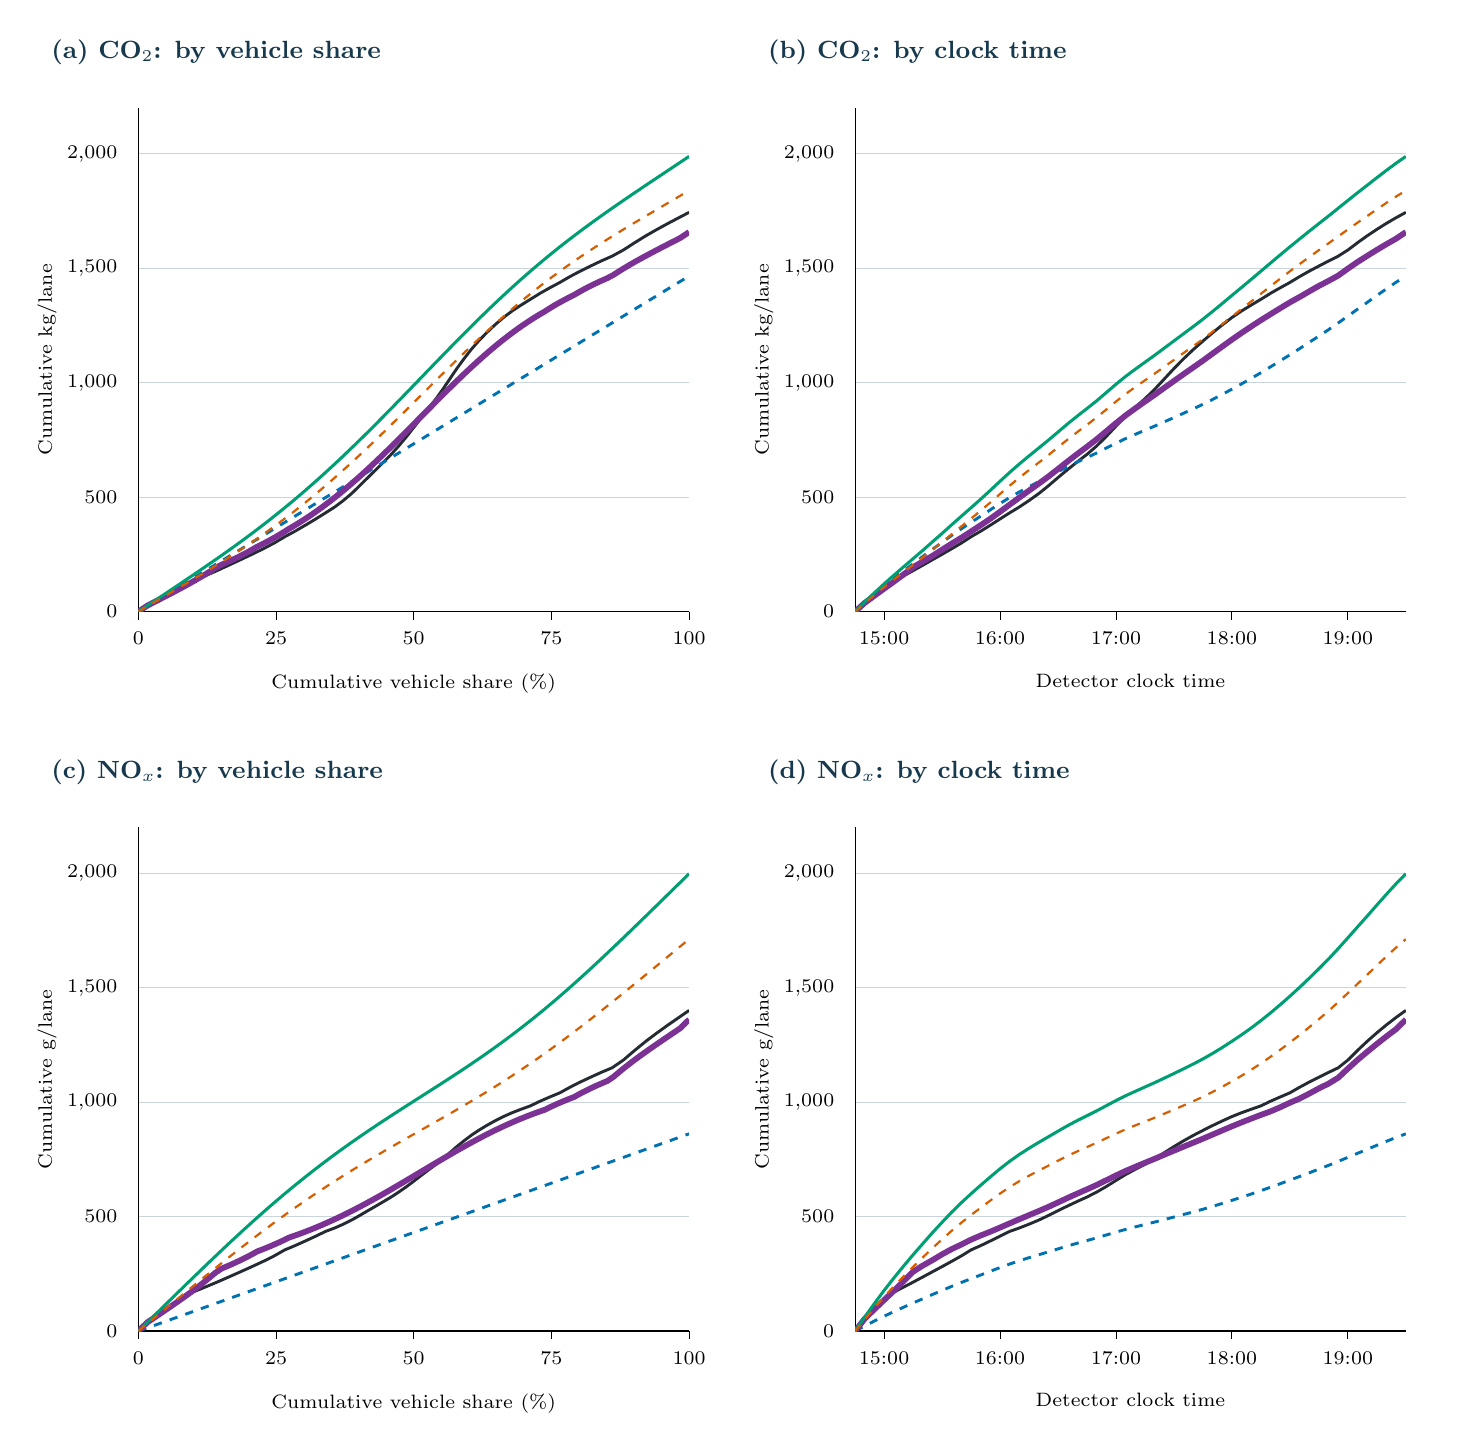
\begin{tikzpicture}[x=1pt,y=1pt]
\useasboundingbox (0,0) rectangle (509,500);
\node[anchor=west,font=\small\bfseries,text=navy] at (5,491) {(a) CO$_2$: by vehicle share};
\draw[rulegray,line width=.25pt] (40,289.000) -- (239,289.000);
\node[anchor=east,font=\scriptsize] at (36,289.000) {0};
\draw[rulegray,line width=.25pt] (40,330.364) -- (239,330.364);
\node[anchor=east,font=\scriptsize] at (36,330.364) {500};
\draw[rulegray,line width=.25pt] (40,371.727) -- (239,371.727);
\node[anchor=east,font=\scriptsize] at (36,371.727) {1,000};
\draw[rulegray,line width=.25pt] (40,413.091) -- (239,413.091);
\node[anchor=east,font=\scriptsize] at (36,413.091) {1,500};
\draw[rulegray,line width=.25pt] (40,454.455) -- (239,454.455);
\node[anchor=east,font=\scriptsize] at (36,454.455) {2,000};
\draw[black,line width=.35pt] (40.000,289) -- (40.000,286);
\node[anchor=north,font=\scriptsize] at (40.000,285) {0};
\draw[black,line width=.35pt] (89.750,289) -- (89.750,286);
\node[anchor=north,font=\scriptsize] at (89.750,285) {25};
\draw[black,line width=.35pt] (139.500,289) -- (139.500,286);
\node[anchor=north,font=\scriptsize] at (139.500,285) {50};
\draw[black,line width=.35pt] (189.250,289) -- (189.250,286);
\node[anchor=north,font=\scriptsize] at (189.250,285) {75};
\draw[black,line width=.35pt] (239.000,289) -- (239.000,286);
\node[anchor=north,font=\scriptsize] at (239.000,285) {100};
\draw[black,line width=.45pt] (40,471) -- (40,289) -- (239,289);
\node[anchor=north,font=\scriptsize] at (139.5,270) {Cumulative vehicle share (\%)};
\node[rotate=90,font=\scriptsize] at (7,380.0) {Cumulative kg/lane};
\begin{scope}
\clip (40,289) rectangle (239,471);
\draw[methodO,line width=1.05pt,] plot coordinates {(40.000,289.000) (45.216,292.315) (50.212,294.946) (55.041,297.532) (59.607,299.977) (64.049,301.874) (68.392,303.785) (72.641,305.741) (76.916,307.732) (81.045,309.693) (85.172,311.708) (89.099,313.772) (92.904,316.038) (96.631,318.055) (100.375,320.234) (104.109,322.473) (107.659,324.694) (110.974,326.802) (114.063,329.128) (117.019,331.626) (119.943,334.440) (122.942,337.437) (125.913,340.341) (128.698,343.119) (131.366,345.819) (134.071,348.842) (136.980,352.294) (139.871,356.001) (142.622,359.630) (145.131,362.839) (147.571,365.918) (149.993,369.301) (152.539,373.063) (155.077,376.824) (157.665,380.360) (160.250,383.691) (162.934,386.759) (165.817,389.737) (168.815,392.580) (171.924,395.258) (175.062,397.625) (178.312,399.768) (181.680,401.850) (185.165,404.017) (188.696,406.004) (192.306,407.930) (195.944,410.044) (199.659,412.015) (203.401,413.858) (207.207,415.679) (211.191,417.439) (215.249,419.644) (219.341,422.292) (223.365,424.785) (227.456,427.118) (231.466,429.310) (235.359,431.351) (239.000,433.259)};
\draw[methodS,line width=1.05pt,dashed] plot coordinates {(40.000,289.000) (239.000,410.247)};
\draw[methodR,line width=1.05pt,line width=2.1pt] plot coordinates {(40.000,289.000) (40.005,289.003) (40.017,289.011) (40.035,289.023) (40.060,289.040) (40.091,289.061) (40.130,289.086) (40.174,289.116) (40.226,289.150) (40.284,289.189) (40.349,289.232) (40.420,289.279) (40.498,289.331) (40.582,289.387) (40.673,289.448) (40.771,289.513) (40.876,289.582) (40.986,289.656) (41.104,289.734) (41.228,289.817) (41.359,289.904) (41.496,289.995) (41.640,290.091) (41.790,290.191) (41.947,290.295) (42.110,290.404) (42.280,290.517) (42.456,290.634) (42.639,290.756) (42.828,290.882) (43.024,291.012) (43.226,291.146) (43.434,291.253) (43.649,291.363) (43.871,291.476) (44.099,291.593) (44.333,291.713) (44.573,291.836) (44.820,291.962) (45.074,292.092) (45.333,292.225) (45.599,292.361) (45.871,292.501) (46.150,292.643) (46.435,292.789) (46.726,292.939) (47.023,293.091) (47.326,293.247) (47.636,293.406) (47.952,293.569) (48.274,293.734) (48.602,293.904) (48.937,294.076) (49.277,294.252) (49.624,294.431) (49.976,294.613) (50.335,294.799) (50.700,294.989) (51.071,295.181) (51.448,295.378) (51.830,295.577) (52.219,295.781) (52.614,295.988) (53.015,296.199) (53.422,296.413) (53.834,296.631) (54.253,296.853) (54.677,297.079) (55.108,297.309) (55.544,297.543) (55.986,297.781) (56.434,298.024) (56.887,298.270) (57.347,298.521) (57.812,298.777) (58.283,299.037) (58.759,299.302) (59.241,299.572) (59.729,299.847) (60.223,300.127) (60.722,300.413) (61.227,300.704) (61.738,301.001) (62.254,301.303) (62.776,301.612) (63.303,301.927) (63.835,302.248) (64.374,302.576) (64.917,302.911) (65.466,303.252) (66.021,303.602) (66.581,303.958) (67.146,304.323) (67.716,304.695) (68.292,304.997) (68.873,305.305) (69.460,305.621) (70.051,305.943) (70.648,306.199) (71.250,306.461) (71.857,306.730) (72.470,307.005) (73.087,307.286) (73.709,307.574) (74.337,307.870) (74.969,308.172) (75.606,308.482) (76.248,308.800) (76.895,309.126) (77.547,309.460) (78.203,309.802) (78.864,310.153) (79.530,310.513) (80.200,310.882) (80.875,311.260) (81.555,311.648) (82.239,312.046) (82.927,312.453) (83.620,312.791) (84.317,313.137) (85.019,313.491) (85.724,313.855) (86.434,314.227) (87.148,314.609) (87.866,315.000) (88.588,315.401) (89.313,315.811) (90.043,316.231) (90.776,316.661) (91.514,317.101) (92.254,317.552) (92.999,318.013) (93.747,318.485) (94.498,318.967) (95.253,319.402) (96.011,319.847) (96.772,320.302) (97.537,320.766) (98.304,321.240) (99.075,321.724) (99.848,322.219) (100.624,322.723) (101.404,323.237) (102.185,323.761) (102.970,324.296) (103.757,324.840) (104.546,325.395) (105.338,325.959) (106.132,326.534) (106.928,327.118) (107.726,327.713) (108.527,328.317) (109.329,328.931) (110.133,329.555) (110.939,330.189) (111.747,330.832) (112.556,331.484) (113.367,332.146) (114.179,332.816) (114.993,333.496) (115.808,334.184) (116.624,334.881) (117.441,335.586) (118.259,336.300) (119.078,337.021) (119.898,337.751) (120.719,338.487) (121.540,339.231) (122.362,339.982) (123.184,340.740) (124.007,341.504) (124.831,342.275) (125.654,343.051) (126.478,343.833) (127.301,344.620) (128.125,345.413) (128.949,346.210) (129.773,347.011) (130.596,347.816) (131.419,348.626) (132.242,349.438) (133.064,350.254) (133.886,351.072) (134.708,351.892) (135.528,352.715) (136.348,353.539) (137.168,354.365) (137.986,355.191) (138.804,356.018) (139.621,356.845) (140.436,357.672) (141.251,358.499) (142.065,359.325) (142.877,360.149) (143.688,360.972) (144.498,361.793) (145.307,362.612) (146.114,363.429) (146.920,364.242) (147.724,365.053) (148.527,365.860) (149.328,366.663) (150.128,367.461) (150.926,368.256) (151.722,369.046) (152.517,369.830) (153.310,370.610) (154.101,371.384) (154.890,372.152) (155.678,372.913) (156.463,373.669) (157.247,374.418) (158.028,375.160) (158.808,375.895) (159.586,376.623) (160.362,377.344) (161.135,378.056) (161.907,378.761) (162.676,379.458) (163.444,380.147) (164.209,380.828) (164.972,381.500) (165.733,382.163) (166.491,382.818) (167.248,383.464) (168.002,384.101) (168.753,384.729) (169.503,385.348) (170.250,385.958) (170.995,386.558) (171.738,387.149) (172.478,387.731) (173.216,388.303) (173.951,388.866) (174.684,389.420) (175.414,389.964) (176.143,390.498) (176.868,391.023) (177.591,391.539) (178.312,392.045) (179.030,392.542) (179.746,393.029) (180.459,393.507) (181.169,393.976) (181.877,394.436) (182.582,394.886) (183.284,395.328) (183.984,395.760) (184.681,396.184) (185.376,396.598) (186.068,397.004) (186.757,397.402) (187.443,397.842) (188.126,398.273) (188.807,398.695) (189.484,399.107) (190.159,399.510) (190.831,399.904) (191.500,400.289) (192.166,400.666) (192.829,401.034) (193.489,401.393) (194.146,401.744) (194.800,402.087) (195.451,402.423) (196.098,402.750) (196.742,403.070) (197.383,403.382) (198.021,403.760) (198.656,404.129) (199.287,404.489) (199.915,404.841) (200.539,405.184) (201.160,405.520) (201.778,405.848) (202.392,406.168) (203.002,406.480) (203.609,406.786) (204.212,407.084) (204.811,407.376) (205.406,407.661) (205.998,407.940) (206.586,408.212) (207.170,408.479) (207.750,408.739) (208.326,408.994) (208.899,409.243) (209.467,409.487) (210.031,409.794) (210.590,410.095) (211.146,410.390) (211.697,410.678) (212.244,411.036) (212.787,411.386) (213.325,411.728) (213.859,412.065) (214.388,412.394) (214.913,412.717) (215.433,413.034) (215.949,413.345) (216.460,413.650) (216.966,413.950) (217.467,414.244) (217.964,414.532) (218.456,414.816) (218.942,415.094) (219.424,415.368) (219.901,415.636) (220.373,415.900) (220.840,416.160) (221.301,416.415) (221.757,416.666) (222.209,416.913) (222.655,417.155) (223.095,417.394) (223.530,417.628) (223.960,417.859) (224.385,418.085) (224.804,418.308) (225.217,418.528) (225.625,418.744) (226.028,418.956) (226.425,419.164) (226.816,419.369) (227.201,419.571) (227.581,419.769) (227.955,419.964) (228.323,420.155) (228.685,420.343) (229.042,420.528) (229.393,420.710) (229.737,420.888) (230.076,421.063) (230.409,421.234) (230.736,421.403) (231.057,421.568) (231.372,421.730) (231.680,421.888) (231.983,422.044) (232.279,422.196) (232.570,422.345) (232.854,422.491) (233.132,422.633) (233.404,422.772) (233.669,422.908) (233.928,423.041) (234.181,423.171) (234.428,423.297) (234.668,423.420) (234.902,423.540) (235.130,423.656) (235.351,423.769) (235.566,423.879) (235.775,423.986) (235.977,424.120) (236.172,424.251) (236.361,424.377) (236.544,424.498) (236.720,424.615) (236.890,424.728) (237.054,424.837) (237.210,424.941) (237.361,425.041) (237.504,425.137) (237.641,425.228) (237.772,425.315) (237.896,425.398) (238.014,425.476) (238.124,425.550) (238.229,425.619) (238.327,425.684) (238.418,425.745) (238.502,425.801) (238.580,425.853) (238.651,425.900) (238.716,425.943) (238.774,425.982) (238.826,426.016) (238.870,426.046) (238.909,426.071) (238.940,426.092) (238.965,426.109) (238.983,426.121) (238.995,426.129) (239.000,426.132)};
\draw[methodM,line width=1.05pt,line width=1.1pt] plot coordinates {(40.000,289.000) (40.005,289.003) (40.017,289.011) (40.035,289.023) (40.060,289.040) (40.091,289.061) (40.130,289.086) (40.174,289.116) (40.226,289.150) (40.284,289.189) (40.349,289.232) (40.420,289.279) (40.498,289.331) (40.582,289.387) (40.673,289.448) (40.771,289.513) (40.876,289.582) (40.986,289.656) (41.104,289.734) (41.228,289.817) (41.359,289.904) (41.496,289.995) (41.640,290.091) (41.790,290.191) (41.947,290.295) (42.110,290.404) (42.280,290.517) (42.456,290.634) (42.639,290.756) (42.828,290.881) (43.024,291.012) (43.226,291.146) (43.434,291.285) (43.649,291.428) (43.871,291.575) (44.099,291.727) (44.333,291.883) (44.573,292.043) (44.820,292.207) (45.074,292.376) (45.333,292.548) (45.599,292.725) (45.871,292.907) (46.150,293.092) (46.435,293.281) (46.726,293.475) (47.023,293.673) (47.326,293.875) (47.636,294.081) (47.952,294.292) (48.274,294.506) (48.602,294.725) (48.937,294.947) (49.277,295.174) (49.624,295.405) (49.976,295.640) (50.335,295.880) (50.700,296.123) (51.071,296.370) (51.448,296.622) (51.830,296.877) (52.219,297.137) (52.614,297.401) (53.015,297.668) (53.422,297.940) (53.834,298.216) (54.253,298.496) (54.677,298.781) (55.108,299.069) (55.544,299.361) (55.986,299.658) (56.434,299.959) (56.887,300.263) (57.347,300.572) (57.812,300.885) (58.283,301.203) (58.759,301.524) (59.241,301.850) (59.729,302.180) (60.223,302.514) (60.722,302.852) (61.227,303.195) (61.738,303.542) (62.254,303.893) (62.776,304.249) (63.303,304.609) (63.835,304.973) (64.374,305.342) (64.917,305.715) (65.466,306.093) (66.021,306.475) (66.581,306.862) (67.146,307.254) (67.716,307.650) (68.292,308.051) (68.873,308.456) (69.460,308.867) (70.051,309.282) (70.648,309.702) (71.250,310.127) (71.857,310.557) (72.470,310.992) (73.087,311.432) (73.709,311.877) (74.337,312.327) (74.969,312.782) (75.606,313.243) (76.248,313.709) (76.895,314.180) (77.547,314.657) (78.203,315.139) (78.864,315.627) (79.530,316.121) (80.200,316.620) (80.875,317.124) (81.555,317.635) (82.239,318.151) (82.927,318.673) (83.620,319.200) (84.317,319.734) (85.019,320.274) (85.724,320.820) (86.434,321.372) (87.148,321.930) (87.866,322.494) (88.588,323.064) (89.313,323.640) (90.043,324.223) (90.776,324.812) (91.514,325.407) (92.254,326.009) (92.999,326.616) (93.747,327.231) (94.498,327.851) (95.253,328.478) (96.011,329.111) (96.772,329.751) (97.537,330.397) (98.304,331.049) (99.075,331.708) (99.848,332.373) (100.624,333.044) (101.404,333.722) (102.185,334.406) (102.970,335.096) (103.757,335.792) (104.546,336.494) (105.338,337.202) (106.132,337.917) (106.928,338.637) (107.726,339.363) (108.527,340.095) (109.329,340.832) (110.133,341.575) (110.939,342.324) (111.747,343.077) (112.556,343.837) (113.367,344.601) (114.179,345.370) (114.993,346.145) (115.808,346.924) (116.624,347.708) (117.441,348.496) (118.259,349.289) (119.078,350.086) (119.898,350.887) (120.719,351.692) (121.540,352.501) (122.362,353.314) (123.184,354.130) (124.007,354.949) (124.831,355.771) (125.654,356.597) (126.478,357.425) (127.301,358.255) (128.125,359.088) (128.949,359.923) (129.773,360.760) (130.596,361.599) (131.419,362.440) (132.242,363.281) (133.064,364.124) (133.886,364.968) (134.708,365.813) (135.528,366.658) (136.348,367.504) (137.168,368.350) (137.986,369.196) (138.804,370.042) (139.621,370.887) (140.436,371.732) (141.251,372.576) (142.065,373.418) (142.877,374.260) (143.688,375.100) (144.498,375.939) (145.307,376.776) (146.114,377.611) (146.920,378.443) (147.724,379.274) (148.527,380.102) (149.328,380.927) (150.128,381.750) (150.926,382.569) (151.722,383.385) (152.517,384.198) (153.310,385.008) (154.101,385.814) (154.890,386.616) (155.678,387.414) (156.463,388.209) (157.247,388.999) (158.028,389.785) (158.808,390.566) (159.586,391.343) (160.362,392.115) (161.135,392.883) (161.907,393.645) (162.676,394.403) (163.444,395.156) (164.209,395.904) (164.972,396.646) (165.733,397.383) (166.491,398.115) (167.248,398.842) (168.002,399.563) (168.753,400.279) (169.503,400.989) (170.250,401.693) (170.995,402.392) (171.738,403.085) (172.478,403.772) (173.216,404.454) (173.951,405.130) (174.684,405.800) (175.414,406.464) (176.143,407.123) (176.868,407.776) (177.591,408.422) (178.312,409.064) (179.030,409.699) (179.746,410.328) (180.459,410.952) (181.169,411.570) (181.877,412.182) (182.582,412.788) (183.284,413.388) (183.984,413.983) (184.681,414.573) (185.376,415.156) (186.068,415.734) (186.757,416.306) (187.443,416.873) (188.126,417.434) (188.807,417.990) (189.484,418.540) (190.159,419.085) (190.831,419.625) (191.500,420.159) (192.166,420.688) (192.829,421.211) (193.489,421.730) (194.146,422.243) (194.800,422.752) (195.451,423.255) (196.098,423.753) (196.742,424.247) (197.383,424.735) (198.021,425.219) (198.656,425.698) (199.287,426.172) (199.915,426.641) (200.539,427.106) (201.160,427.566) (201.778,428.021) (202.392,428.472) (203.002,428.919) (203.609,429.361) (204.212,429.799) (204.811,430.232) (205.406,430.661) (205.998,431.086) (206.586,431.506) (207.170,431.922) (207.750,432.334) (208.326,432.742) (208.899,433.146) (209.467,433.546) (210.031,433.942) (210.590,434.334) (211.146,434.721) (211.697,435.105) (212.244,435.485) (212.787,435.861) (213.325,436.233) (213.859,436.601) (214.388,436.965) (214.913,437.325) (215.433,437.682) (215.949,438.035) (216.460,438.383) (216.966,438.729) (217.467,439.070) (217.964,439.407) (218.456,439.741) (218.942,440.071) (219.424,440.397) (219.901,440.719) (220.373,441.038) (220.840,441.353) (221.301,441.664) (221.757,441.971) (222.209,442.274) (222.655,442.574) (223.095,442.870) (223.530,443.162) (223.960,443.450) (224.385,443.734) (224.804,444.015) (225.217,444.292) (225.625,444.565) (226.028,444.834) (226.425,445.099) (226.816,445.360) (227.201,445.617) (227.581,445.871) (227.955,446.120) (228.323,446.366) (228.685,446.608) (229.042,446.845) (229.393,447.079) (229.737,447.309) (230.076,447.535) (230.409,447.756) (230.736,447.974) (231.057,448.188) (231.372,448.397) (231.680,448.603) (231.983,448.804) (232.279,449.002) (232.570,449.195) (232.854,449.384) (233.132,449.569) (233.404,449.750) (233.669,449.927) (233.928,450.099) (234.181,450.268) (234.428,450.432) (234.668,450.592) (234.902,450.747) (235.130,450.899) (235.351,451.046) (235.566,451.189) (235.775,451.328) (235.977,451.462) (236.172,451.592) (236.361,451.718) (236.544,451.840) (236.720,451.957) (236.890,452.070) (237.054,452.179) (237.210,452.283) (237.361,452.383) (237.504,452.478) (237.641,452.570) (237.772,452.657) (237.896,452.739) (238.014,452.817) (238.124,452.891) (238.229,452.961) (238.327,453.026) (238.418,453.086) (238.502,453.142) (238.580,453.194) (238.651,453.242) (238.716,453.285) (238.774,453.323) (238.826,453.358) (238.870,453.387) (238.909,453.413) (238.940,453.434) (238.965,453.450) (238.983,453.463) (238.995,453.470) (239.000,453.474)};
\draw[methodA,line width=1.05pt,dashed,line width=.8pt] plot coordinates {(40.000,289.000) (40.005,289.003) (40.017,289.010) (40.035,289.020) (40.060,289.035) (40.091,289.054) (40.130,289.076) (40.174,289.102) (40.226,289.132) (40.284,289.166) (40.349,289.204) (40.420,289.246) (40.498,289.292) (40.582,289.342) (40.673,289.395) (40.771,289.452) (40.876,289.513) (40.986,289.579) (41.104,289.647) (41.228,289.720) (41.359,289.797) (41.496,289.877) (41.640,289.962) (41.790,290.050) (41.947,290.142) (42.110,290.237) (42.280,290.337) (42.456,290.440) (42.639,290.548) (42.828,290.659) (43.024,290.773) (43.226,290.892) (43.434,291.014) (43.649,291.140) (43.871,291.270) (44.099,291.404) (44.333,291.541) (44.573,291.682) (44.820,291.827) (45.074,291.976) (45.333,292.128) (45.599,292.284) (45.871,292.444) (46.150,292.607) (46.435,292.774) (46.726,292.945) (47.023,293.119) (47.326,293.298) (47.636,293.479) (47.952,293.665) (48.274,293.854) (48.602,294.047) (48.937,294.243) (49.277,294.443) (49.624,294.647) (49.976,294.854) (50.335,295.065) (50.700,295.280) (51.071,295.498) (51.448,295.720) (51.830,295.945) (52.219,296.174) (52.614,296.407) (53.015,296.643) (53.422,296.883) (53.834,297.127) (54.253,297.374) (54.677,297.625) (55.108,297.880) (55.544,298.138) (55.986,298.400) (56.434,298.666) (56.887,298.935) (57.347,299.208) (57.812,299.485) (58.283,299.765) (58.759,300.050) (59.241,300.338) (59.729,300.630) (60.223,300.926) (60.722,301.225) (61.227,301.529) (61.738,301.836) (62.254,302.148) (62.776,302.463) (63.303,302.782) (63.835,303.106) (64.374,303.433) (64.917,303.765) (65.466,304.101) (66.021,304.441) (66.581,304.785) (67.146,305.134) (67.716,305.487) (68.292,305.844) (68.873,306.206) (69.460,306.572) (70.051,306.943) (70.648,307.318) (71.250,307.698) (71.857,308.083) (72.470,308.472) (73.087,308.867) (73.709,309.266) (74.337,309.670) (74.969,310.079) (75.606,310.494) (76.248,310.913) (76.895,311.338) (77.547,311.768) (78.203,312.203) (78.864,312.643) (79.530,313.089) (80.200,313.541) (80.875,313.998) (81.555,314.461) (82.239,314.930) (82.927,315.404) (83.620,315.884) (84.317,316.370) (85.019,316.863) (85.724,317.361) (86.434,317.865) (87.148,318.375) (87.866,318.892) (88.588,319.414) (89.313,319.943) (90.043,320.479) (90.776,321.020) (91.514,321.568) (92.254,322.123) (92.999,322.684) (93.747,323.251) (94.498,323.825) (95.253,324.405) (96.011,324.992) (96.772,325.586) (97.537,326.186) (98.304,326.793) (99.075,327.406) (99.848,328.025) (100.624,328.652) (101.404,329.284) (102.185,329.924) (102.970,330.569) (103.757,331.221) (104.546,331.880) (105.338,332.545) (106.132,333.216) (106.928,333.893) (107.726,334.576) (108.527,335.266) (109.329,335.961) (110.133,336.663) (110.939,337.370) (111.747,338.082) (112.556,338.801) (113.367,339.525) (114.179,340.254) (114.993,340.989) (115.808,341.728) (116.624,342.473) (117.441,343.223) (118.259,343.977) (119.078,344.736) (119.898,345.499) (120.719,346.266) (121.540,347.038) (122.362,347.813) (123.184,348.592) (124.007,349.375) (124.831,350.161) (125.654,350.950) (126.478,351.743) (127.301,352.538) (128.125,353.335) (128.949,354.135) (129.773,354.938) (130.596,355.742) (131.419,356.548) (132.242,357.356) (133.064,358.165) (133.886,358.975) (134.708,359.786) (135.528,360.598) (136.348,361.410) (137.168,362.223) (137.986,363.036) (138.804,363.849) (139.621,364.661) (140.436,365.473) (141.251,366.284) (142.065,367.094) (142.877,367.903) (143.688,368.711) (144.498,369.517) (145.307,370.321) (146.114,371.124) (146.920,371.924) (147.724,372.722) (148.527,373.517) (149.328,374.310) (150.128,375.099) (150.926,375.886) (151.722,376.669) (152.517,377.449) (153.310,378.226) (154.101,378.999) (154.890,379.767) (155.678,380.532) (156.463,381.293) (157.247,382.049) (158.028,382.801) (158.808,383.549) (159.586,384.291) (160.362,385.029) (161.135,385.762) (161.907,386.490) (162.676,387.213) (163.444,387.930) (164.209,388.643) (164.972,389.349) (165.733,390.051) (166.491,390.747) (167.248,391.437) (168.002,392.121) (168.753,392.800) (169.503,393.473) (170.250,394.140) (170.995,394.802) (171.738,395.457) (172.478,396.106) (173.216,396.750) (173.951,397.387) (174.684,398.018) (175.414,398.644) (176.143,399.263) (176.868,399.876) (177.591,400.483) (178.312,401.084) (179.030,401.680) (179.746,402.269) (180.459,402.851) (181.169,403.428) (181.877,403.999) (182.582,404.564) (183.284,405.123) (183.984,405.677) (184.681,406.224) (185.376,406.765) (186.068,407.301) (186.757,407.831) (187.443,408.355) (188.126,408.873) (188.807,409.386) (189.484,409.893) (190.159,410.395) (190.831,410.891) (191.500,411.382) (192.166,411.868) (192.829,412.348) (193.489,412.822) (194.146,413.292) (194.800,413.756) (195.451,414.216) (196.098,414.670) (196.742,415.119) (197.383,415.564) (198.021,416.003) (198.656,416.438) (199.287,416.868) (199.915,417.293) (200.539,417.714) (201.160,418.130) (201.778,418.541) (202.392,418.948) (203.002,419.351) (203.609,419.749) (204.212,420.143) (204.811,420.533) (205.406,420.918) (205.998,421.299) (206.586,421.677) (207.170,422.050) (207.750,422.419) (208.326,422.784) (208.899,423.145) (209.467,423.502) (210.031,423.856) (210.590,424.205) (211.146,424.551) (211.697,424.893) (212.244,425.232) (212.787,425.566) (213.325,425.897) (213.859,426.225) (214.388,426.548) (214.913,426.869) (215.433,427.185) (215.949,427.498) (216.460,427.808) (216.966,428.114) (217.467,428.416) (217.964,428.715) (218.456,429.011) (218.942,429.303) (219.424,429.592) (219.901,429.877) (220.373,430.159) (220.840,430.437) (221.301,430.712) (221.757,430.984) (222.209,431.252) (222.655,431.517) (223.095,431.778) (223.530,432.036) (223.960,432.291) (224.385,432.542) (224.804,432.790) (225.217,433.034) (225.625,433.275) (226.028,433.512) (226.425,433.746) (226.816,433.977) (227.201,434.204) (227.581,434.428) (227.955,434.648) (228.323,434.864) (228.685,435.078) (229.042,435.287) (229.393,435.493) (229.737,435.696) (230.076,435.895) (230.409,436.091) (230.736,436.282) (231.057,436.471) (231.372,436.656) (231.680,436.837) (231.983,437.015) (232.279,437.189) (232.570,437.359) (232.854,437.526) (233.132,437.689) (233.404,437.848) (233.669,438.004) (233.928,438.156) (234.181,438.304) (234.428,438.449) (234.668,438.590) (234.902,438.727) (235.130,438.861) (235.351,438.991) (235.566,439.117) (235.775,439.239) (235.977,439.357) (236.172,439.472) (236.361,439.583) (236.544,439.690) (236.720,439.794) (236.890,439.893) (237.054,439.989) (237.210,440.081) (237.361,440.169) (237.504,440.253) (237.641,440.334) (237.772,440.410) (237.896,440.483) (238.014,440.552) (238.124,440.617) (238.229,440.678) (238.327,440.736) (238.418,440.789) (238.502,440.839) (238.580,440.884) (238.651,440.926) (238.716,440.964) (238.774,440.998) (238.826,441.028) (238.870,441.055) (238.909,441.077) (238.940,441.095) (238.965,441.110) (238.983,441.121) (238.995,441.128) (239.000,441.131)};
\end{scope}
\node[anchor=west,font=\small\bfseries,text=navy] at (264,491) {(b) CO$_2$: by clock time};
\draw[rulegray,line width=.25pt] (299,289.000) -- (498,289.000);
\node[anchor=east,font=\scriptsize] at (295,289.000) {0};
\draw[rulegray,line width=.25pt] (299,330.364) -- (498,330.364);
\node[anchor=east,font=\scriptsize] at (295,330.364) {500};
\draw[rulegray,line width=.25pt] (299,371.727) -- (498,371.727);
\node[anchor=east,font=\scriptsize] at (295,371.727) {1,000};
\draw[rulegray,line width=.25pt] (299,413.091) -- (498,413.091);
\node[anchor=east,font=\scriptsize] at (295,413.091) {1,500};
\draw[rulegray,line width=.25pt] (299,454.455) -- (498,454.455);
\node[anchor=east,font=\scriptsize] at (295,454.455) {2,000};
\draw[black,line width=.35pt] (309.474,289) -- (309.474,286);
\node[anchor=north,font=\scriptsize] at (309.474,285) {15:00};
\draw[black,line width=.35pt] (351.368,289) -- (351.368,286);
\node[anchor=north,font=\scriptsize] at (351.368,285) {16:00};
\draw[black,line width=.35pt] (393.263,289) -- (393.263,286);
\node[anchor=north,font=\scriptsize] at (393.263,285) {17:00};
\draw[black,line width=.35pt] (435.158,289) -- (435.158,286);
\node[anchor=north,font=\scriptsize] at (435.158,285) {18:00};
\draw[black,line width=.35pt] (477.053,289) -- (477.053,286);
\node[anchor=north,font=\scriptsize] at (477.053,285) {19:00};
\draw[black,line width=.45pt] (299,471) -- (299,289) -- (498,289);
\node[anchor=north,font=\scriptsize] at (398.5,270) {Detector clock time};
\node[rotate=90,font=\scriptsize] at (266,380.0) {Cumulative kg/lane};
\begin{scope}
\clip (299,289) rectangle (498,471);
\draw[methodO,line width=1.05pt,] plot coordinates {(299.000,289.000) (302.491,292.315) (305.982,294.946) (309.474,297.532) (312.965,299.977) (316.456,301.874) (319.947,303.785) (323.439,305.741) (326.930,307.732) (330.421,309.693) (333.912,311.708) (337.404,313.772) (340.895,316.038) (344.386,318.055) (347.877,320.234) (351.368,322.473) (354.860,324.694) (358.351,326.802) (361.842,329.128) (365.333,331.626) (368.825,334.440) (372.316,337.437) (375.807,340.341) (379.298,343.119) (382.789,345.819) (386.281,348.842) (389.772,352.294) (393.263,356.001) (396.754,359.630) (400.246,362.839) (403.737,365.918) (407.228,369.301) (410.719,373.063) (414.211,376.824) (417.702,380.360) (421.193,383.691) (424.684,386.759) (428.175,389.737) (431.667,392.580) (435.158,395.258) (438.649,397.625) (442.140,399.768) (445.632,401.850) (449.123,404.017) (452.614,406.004) (456.105,407.930) (459.596,410.044) (463.088,412.015) (466.579,413.858) (470.070,415.679) (473.561,417.439) (477.053,419.644) (480.544,422.292) (484.035,424.785) (487.526,427.118) (491.018,429.310) (494.509,431.351) (498.000,433.259)};
\draw[methodS,line width=1.05pt,dashed] plot coordinates {(299.000,289.000) (302.491,292.178) (305.982,295.222) (309.474,298.164) (312.965,300.946) (316.456,303.652) (319.947,306.299) (323.439,308.888) (326.930,311.492) (330.421,314.008) (333.912,316.522) (337.404,318.915) (340.895,321.233) (344.386,323.504) (347.877,325.786) (351.368,328.060) (354.860,330.223) (358.351,332.243) (361.842,334.125) (365.333,335.926) (368.825,337.708) (372.316,339.535) (375.807,341.345) (379.298,343.042) (382.789,344.668) (386.281,346.316) (389.772,348.088) (393.263,349.850) (396.754,351.526) (400.246,353.055) (403.737,354.541) (407.228,356.017) (410.719,357.568) (414.211,359.114) (417.702,360.691) (421.193,362.266) (424.684,363.902) (428.175,365.658) (431.667,367.485) (435.158,369.379) (438.649,371.291) (442.140,373.271) (445.632,375.323) (449.123,377.447) (452.614,379.598) (456.105,381.797) (459.596,384.014) (463.088,386.278) (466.579,388.557) (470.070,390.877) (473.561,393.304) (477.053,395.776) (480.544,398.269) (484.035,400.721) (487.526,403.214) (491.018,405.657) (494.509,408.029) (498.000,410.247)};
\draw[methodR,line width=1.05pt,line width=2.1pt] plot coordinates {(299.000,289.000) (302.491,292.165) (305.982,294.735) (309.474,297.273) (312.965,299.778) (316.456,302.378) (319.947,305.050) (323.439,307.083) (326.930,309.137) (330.421,311.357) (333.912,313.570) (337.404,315.690) (340.895,317.954) (344.386,320.217) (347.877,322.561) (351.368,325.087) (354.860,327.662) (358.351,330.216) (361.842,332.720) (365.333,335.222) (368.825,337.791) (372.316,340.516) (375.807,343.297) (379.298,345.967) (382.789,348.574) (386.281,351.257) (389.772,354.175) (393.263,357.099) (396.754,359.891) (400.246,362.435) (403.737,364.899) (407.228,367.327) (410.719,369.853) (414.211,372.332) (417.702,374.815) (421.193,377.240) (424.684,379.690) (428.175,382.236) (431.667,384.779) (435.158,387.296) (438.649,389.701) (442.140,392.045) (445.632,394.308) (449.123,396.472) (452.614,398.626) (456.105,400.743) (459.596,402.672) (463.088,404.698) (466.579,406.681) (470.070,408.495) (473.561,410.413) (477.053,412.922) (480.544,415.320) (484.035,417.539) (487.526,419.704) (491.018,421.778) (494.509,423.773) (498.000,426.132)};
\draw[methodM,line width=1.05pt,line width=1.1pt] plot coordinates {(299.000,289.000) (302.491,292.471) (305.982,295.798) (309.474,299.024) (312.965,302.097) (316.456,305.119) (319.947,308.120) (323.439,311.114) (326.930,314.196) (330.421,317.252) (333.912,320.392) (337.404,323.470) (340.895,326.539) (344.386,329.633) (347.877,332.829) (351.368,336.105) (354.860,339.301) (358.351,342.356) (361.842,345.260) (365.333,348.089) (368.825,350.932) (372.316,353.889) (375.807,356.857) (379.298,359.669) (382.789,362.386) (386.281,365.159) (389.772,368.156) (393.263,371.147) (396.754,373.996) (400.246,376.594) (403.737,379.116) (407.228,381.612) (410.719,384.222) (414.211,386.805) (417.702,389.419) (421.193,392.004) (424.684,394.656) (428.175,397.465) (431.667,400.336) (435.158,403.258) (438.649,406.144) (442.140,409.063) (445.632,412.011) (449.123,414.979) (452.614,417.899) (456.105,420.798) (459.596,423.635) (463.088,426.450) (466.579,429.210) (470.070,431.949) (473.561,434.753) (477.053,437.556) (480.544,440.341) (484.035,443.051) (487.526,445.787) (491.018,448.460) (494.509,451.051) (498.000,453.474)};
\draw[methodA,line width=1.05pt,dashed,line width=.8pt] plot coordinates {(299.000,289.000) (302.491,292.059) (305.982,294.993) (309.474,297.840) (312.965,300.556) (316.456,303.236) (319.947,305.906) (323.439,308.582) (326.930,311.351) (330.421,314.114) (333.912,316.971) (337.404,319.787) (340.895,322.612) (344.386,325.476) (347.877,328.450) (351.368,331.515) (354.860,334.518) (358.351,337.400) (361.842,340.149) (365.333,342.835) (368.825,345.541) (372.316,348.362) (375.807,351.199) (379.298,353.892) (382.789,356.496) (386.281,359.158) (389.772,362.037) (393.263,364.911) (396.754,367.650) (400.246,370.147) (403.737,372.570) (407.228,374.967) (410.719,377.472) (414.211,379.949) (417.702,382.451) (421.193,384.923) (424.684,387.454) (428.175,390.128) (431.667,392.855) (435.158,395.620) (438.649,398.342) (442.140,401.084) (445.632,403.841) (449.123,406.601) (452.614,409.303) (456.105,411.969) (459.596,414.562) (463.088,417.120) (466.579,419.613) (470.070,422.073) (473.561,424.579) (477.053,427.073) (480.544,429.542) (484.035,431.939) (487.526,434.354) (491.018,436.711) (494.509,438.995) (498.000,441.131)};
\end{scope}
\node[anchor=west,font=\small\bfseries,text=navy] at (5,231) {(c) NO$_x$: by vehicle share};
\draw[rulegray,line width=.25pt] (40,29.000) -- (239,29.000);
\node[anchor=east,font=\scriptsize] at (36,29.000) {0};
\draw[rulegray,line width=.25pt] (40,70.364) -- (239,70.364);
\node[anchor=east,font=\scriptsize] at (36,70.364) {500};
\draw[rulegray,line width=.25pt] (40,111.727) -- (239,111.727);
\node[anchor=east,font=\scriptsize] at (36,111.727) {1,000};
\draw[rulegray,line width=.25pt] (40,153.091) -- (239,153.091);
\node[anchor=east,font=\scriptsize] at (36,153.091) {1,500};
\draw[rulegray,line width=.25pt] (40,194.455) -- (239,194.455);
\node[anchor=east,font=\scriptsize] at (36,194.455) {2,000};
\draw[black,line width=.35pt] (40.000,29) -- (40.000,26);
\node[anchor=north,font=\scriptsize] at (40.000,25) {0};
\draw[black,line width=.35pt] (89.750,29) -- (89.750,26);
\node[anchor=north,font=\scriptsize] at (89.750,25) {25};
\draw[black,line width=.35pt] (139.500,29) -- (139.500,26);
\node[anchor=north,font=\scriptsize] at (139.500,25) {50};
\draw[black,line width=.35pt] (189.250,29) -- (189.250,26);
\node[anchor=north,font=\scriptsize] at (189.250,25) {75};
\draw[black,line width=.35pt] (239.000,29) -- (239.000,26);
\node[anchor=north,font=\scriptsize] at (239.000,25) {100};
\draw[black,line width=.45pt] (40,211) -- (40,29) -- (239,29);
\node[anchor=north,font=\scriptsize] at (139.5,10) {Cumulative vehicle share (\%)};
\node[rotate=90,font=\scriptsize] at (7,120.0) {Cumulative g/lane};
\begin{scope}
\clip (40,29) rectangle (239,211);
\draw[methodO,line width=1.05pt,] plot coordinates {(40.000,29.000) (45.216,33.370) (50.212,36.698) (55.041,39.971) (59.607,43.065) (64.049,44.869) (68.392,46.687) (72.641,48.548) (76.916,50.442) (81.045,52.307) (85.172,54.224) (89.099,56.188) (92.904,58.344) (96.631,59.904) (100.375,61.588) (104.109,63.319) (107.659,65.036) (110.974,66.276) (114.063,67.643) (117.019,69.112) (119.943,70.767) (122.942,72.529) (125.913,74.237) (128.698,75.870) (131.366,77.458) (134.071,79.235) (136.980,81.265) (139.871,83.445) (142.622,85.578) (145.131,87.465) (147.571,89.276) (149.993,91.265) (152.539,93.477) (155.077,95.689) (157.665,97.768) (160.250,99.726) (162.934,101.530) (165.817,103.281) (168.815,104.953) (171.924,106.527) (175.062,107.919) (178.312,109.179) (181.680,110.404) (185.165,112.079) (188.696,113.615) (192.306,115.105) (195.944,117.115) (199.659,118.991) (203.401,120.743) (207.207,122.477) (211.191,124.151) (215.249,126.940) (219.341,130.431) (223.365,133.716) (227.456,136.792) (231.466,139.681) (235.359,142.371) (239.000,144.886)};
\draw[methodS,line width=1.05pt,dashed] plot coordinates {(40.000,29.000) (239.000,100.293)};
\draw[methodR,line width=1.05pt,line width=2.1pt] plot coordinates {(40.000,29.000) (40.005,29.005) (40.017,29.016) (40.035,29.034) (40.060,29.059) (40.091,29.089) (40.130,29.127) (40.174,29.171) (40.226,29.221) (40.284,29.278) (40.349,29.341) (40.420,29.411) (40.498,29.487) (40.582,29.570) (40.673,29.660) (40.771,29.755) (40.876,29.857) (40.986,29.966) (41.104,30.081) (41.228,30.203) (41.359,30.330) (41.496,30.465) (41.640,30.606) (41.790,30.753) (41.947,30.906) (42.110,31.066) (42.280,31.232) (42.456,31.405) (42.639,31.584) (42.828,31.769) (43.024,31.961) (43.226,32.159) (43.434,32.300) (43.649,32.445) (43.871,32.594) (44.099,32.748) (44.333,32.906) (44.573,33.068) (44.820,33.235) (45.074,33.406) (45.333,33.581) (45.599,33.760) (45.871,33.944) (46.150,34.132) (46.435,34.325) (46.726,34.522) (47.023,34.723) (47.326,34.928) (47.636,35.138) (47.952,35.352) (48.274,35.571) (48.602,35.793) (48.937,36.021) (49.277,36.252) (49.624,36.488) (49.976,36.729) (50.335,36.974) (50.700,37.224) (51.071,37.478) (51.448,37.736) (51.830,38.000) (52.219,38.268) (52.614,38.541) (53.015,38.818) (53.422,39.101) (53.834,39.389) (54.253,39.681) (54.677,39.979) (55.108,40.282) (55.544,40.591) (55.986,40.904) (56.434,41.224) (56.887,41.549) (57.347,41.880) (57.812,42.217) (58.283,42.560) (58.759,42.909) (59.241,43.265) (59.729,43.628) (60.223,43.997) (60.722,44.373) (61.227,44.757) (61.738,45.148) (62.254,45.547) (62.776,45.954) (63.303,46.369) (63.835,46.792) (64.374,47.224) (64.917,47.665) (65.466,48.116) (66.021,48.576) (66.581,49.046) (67.146,49.527) (67.716,50.018) (68.292,50.399) (68.873,50.790) (69.460,51.189) (70.051,51.597) (70.648,51.840) (71.250,52.090) (71.857,52.345) (72.470,52.607) (73.087,52.874) (73.709,53.149) (74.337,53.430) (74.969,53.717) (75.606,54.012) (76.248,54.315) (76.895,54.625) (77.547,54.942) (78.203,55.268) (78.864,55.602) (79.530,55.944) (80.200,56.295) (80.875,56.655) (81.555,57.024) (82.239,57.402) (82.927,57.790) (83.620,58.051) (84.317,58.318) (85.019,58.593) (85.724,58.874) (86.434,59.162) (87.148,59.457) (87.866,59.759) (88.588,60.069) (89.313,60.386) (90.043,60.711) (90.776,61.043) (91.514,61.384) (92.254,61.732) (92.999,62.089) (93.747,62.453) (94.498,62.826) (95.253,63.082) (96.011,63.344) (96.772,63.611) (97.537,63.884) (98.304,64.163) (99.075,64.448) (99.848,64.738) (100.624,65.035) (101.404,65.337) (102.185,65.645) (102.970,65.959) (103.757,66.279) (104.546,66.606) (105.338,66.938) (106.132,67.275) (106.928,67.619) (107.726,67.969) (108.527,68.324) (109.329,68.685) (110.133,69.052) (110.939,69.424) (111.747,69.803) (112.556,70.186) (113.367,70.575) (114.179,70.969) (114.993,71.369) (115.808,71.774) (116.624,72.184) (117.441,72.598) (118.259,73.018) (119.078,73.442) (119.898,73.871) (120.719,74.304) (121.540,74.741) (122.362,75.183) (123.184,75.629) (124.007,76.078) (124.831,76.531) (125.654,76.987) (126.478,77.447) (127.301,77.910) (128.125,78.376) (128.949,78.845) (129.773,79.316) (130.596,79.789) (131.419,80.265) (132.242,80.743) (133.064,81.222) (133.886,81.704) (134.708,82.186) (135.528,82.670) (136.348,83.154) (137.168,83.640) (137.986,84.126) (138.804,84.612) (139.621,85.098) (140.436,85.585) (141.251,86.071) (142.065,86.556) (142.877,87.041) (143.688,87.525) (144.498,88.008) (145.307,88.489) (146.114,88.969) (146.920,89.448) (147.724,89.924) (148.527,90.399) (149.328,90.871) (150.128,91.341) (150.926,91.808) (151.722,92.272) (152.517,92.733) (153.310,93.192) (154.101,93.647) (154.890,94.098) (155.678,94.546) (156.463,94.991) (157.247,95.431) (158.028,95.867) (158.808,96.300) (159.586,96.728) (160.362,97.151) (161.135,97.570) (161.907,97.985) (162.676,98.395) (163.444,98.800) (164.209,99.200) (164.972,99.595) (165.733,99.985) (166.491,100.370) (167.248,100.750) (168.002,101.125) (168.753,101.494) (169.503,101.858) (170.250,102.216) (170.995,102.569) (171.738,102.917) (172.478,103.259) (173.216,103.595) (173.951,103.926) (174.684,104.252) (175.414,104.572) (176.143,104.886) (176.868,105.195) (177.591,105.498) (178.312,105.796) (179.030,106.088) (179.746,106.374) (180.459,106.655) (181.169,106.931) (181.877,107.201) (182.582,107.466) (183.284,107.726) (183.984,107.980) (184.681,108.229) (185.376,108.473) (186.068,108.712) (186.757,108.945) (187.443,109.286) (188.126,109.619) (188.807,109.945) (189.484,110.264) (190.159,110.575) (190.831,110.880) (191.500,111.178) (192.166,111.469) (192.829,111.753) (193.489,112.031) (194.146,112.303) (194.800,112.568) (195.451,112.827) (196.098,113.080) (196.742,113.328) (197.383,113.569) (198.021,113.928) (198.656,114.279) (199.287,114.622) (199.915,114.957) (200.539,115.283) (201.160,115.603) (201.778,115.915) (202.392,116.219) (203.002,116.517) (203.609,116.807) (204.212,117.091) (204.811,117.369) (205.406,117.640) (205.998,117.905) (206.586,118.164) (207.170,118.417) (207.750,118.665) (208.326,118.907) (208.899,119.144) (209.467,119.376) (210.031,119.765) (210.590,120.146) (211.146,120.519) (211.697,120.884) (212.244,121.355) (212.787,121.817) (213.325,122.269) (213.859,122.712) (214.388,123.146) (214.913,123.572) (215.433,123.990) (215.949,124.399) (216.460,124.802) (216.966,125.196) (217.467,125.584) (217.964,125.964) (218.456,126.338) (218.942,126.705) (219.424,127.065) (219.901,127.419) (220.373,127.768) (220.840,128.110) (221.301,128.446) (221.757,128.777) (222.209,129.102) (222.655,129.421) (223.095,129.736) (223.530,130.045) (223.960,130.349) (224.385,130.648) (224.804,130.942) (225.217,131.231) (225.625,131.515) (226.028,131.795) (226.425,132.070) (226.816,132.340) (227.201,132.606) (227.581,132.867) (227.955,133.124) (228.323,133.376) (228.685,133.624) (229.042,133.867) (229.393,134.107) (229.737,134.341) (230.076,134.572) (230.409,134.798) (230.736,135.020) (231.057,135.238) (231.372,135.451) (231.680,135.660) (231.983,135.865) (232.279,136.066) (232.570,136.262) (232.854,136.454) (233.132,136.642) (233.404,136.825) (233.669,137.005) (233.928,137.180) (234.181,137.350) (234.428,137.517) (234.668,137.679) (234.902,137.837) (235.130,137.990) (235.351,138.140) (235.566,138.284) (235.775,138.425) (235.977,138.623) (236.172,138.815) (236.361,139.000) (236.544,139.179) (236.720,139.351) (236.890,139.518) (237.054,139.678) (237.210,139.831) (237.361,139.978) (237.504,140.119) (237.641,140.253) (237.772,140.381) (237.896,140.503) (238.014,140.618) (238.124,140.726) (238.229,140.829) (238.327,140.924) (238.418,141.013) (238.502,141.096) (238.580,141.173) (238.651,141.242) (238.716,141.306) (238.774,141.363) (238.826,141.413) (238.870,141.457) (238.909,141.494) (238.940,141.525) (238.965,141.550) (238.983,141.567) (238.995,141.579) (239.000,141.584)};
\draw[methodM,line width=1.05pt,line width=1.1pt] plot coordinates {(40.000,29.000) (40.005,29.005) (40.017,29.016) (40.035,29.034) (40.060,29.059) (40.091,29.089) (40.130,29.127) (40.174,29.171) (40.226,29.221) (40.284,29.278) (40.349,29.341) (40.420,29.411) (40.498,29.487) (40.582,29.570) (40.673,29.660) (40.771,29.755) (40.876,29.857) (40.986,29.966) (41.104,30.081) (41.228,30.203) (41.359,30.330) (41.496,30.465) (41.640,30.606) (41.790,30.753) (41.947,30.906) (42.110,31.066) (42.280,31.232) (42.456,31.405) (42.639,31.584) (42.828,31.769) (43.024,31.961) (43.226,32.159) (43.434,32.363) (43.649,32.574) (43.871,32.791) (44.099,33.014) (44.333,33.243) (44.573,33.479) (44.820,33.720) (45.074,33.968) (45.333,34.223) (45.599,34.483) (45.871,34.749) (46.150,35.022) (46.435,35.301) (46.726,35.586) (47.023,35.877) (47.326,36.174) (47.636,36.477) (47.952,36.786) (48.274,37.101) (48.602,37.422) (48.937,37.749) (49.277,38.083) (49.624,38.422) (49.976,38.767) (50.335,39.117) (50.700,39.474) (51.071,39.837) (51.448,40.205) (51.830,40.579) (52.219,40.959) (52.614,41.345) (53.015,41.736) (53.422,42.133) (53.834,42.536) (54.253,42.944) (54.677,43.358) (55.108,43.778) (55.544,44.203) (55.986,44.634) (56.434,45.070) (56.887,45.511) (57.347,45.958) (57.812,46.410) (58.283,46.867) (58.759,47.330) (59.241,47.798) (59.729,48.271) (60.223,48.749) (60.722,49.232) (61.227,49.721) (61.738,50.214) (62.254,50.712) (62.776,51.215) (63.303,51.722) (63.835,52.235) (64.374,52.752) (64.917,53.273) (65.466,53.800) (66.021,54.330) (66.581,54.865) (67.146,55.404) (67.716,55.948) (68.292,56.495) (68.873,57.047) (69.460,57.603) (70.051,58.162) (70.648,58.725) (71.250,59.292) (71.857,59.863) (72.470,60.437) (73.087,61.014) (73.709,61.595) (74.337,62.179) (74.969,62.766) (75.606,63.356) (76.248,63.949) (76.895,64.544) (77.547,65.143) (78.203,65.744) (78.864,66.347) (79.530,66.952) (80.200,67.560) (80.875,68.170) (81.555,68.781) (82.239,69.395) (82.927,70.010) (83.620,70.627) (84.317,71.245) (85.019,71.864) (85.724,72.485) (86.434,73.106) (87.148,73.729) (87.866,74.352) (88.588,74.976) (89.313,75.600) (90.043,76.225) (90.776,76.850) (91.514,77.475) (92.254,78.100) (92.999,78.725) (93.747,79.350) (94.498,79.974) (95.253,80.598) (96.011,81.222) (96.772,81.844) (97.537,82.466) (98.304,83.087) (99.075,83.706) (99.848,84.325) (100.624,84.942) (101.404,85.558) (102.185,86.173) (102.970,86.786) (103.757,87.397) (104.546,88.007) (105.338,88.615) (106.132,89.220) (106.928,89.824) (107.726,90.426) (108.527,91.026) (109.329,91.624) (110.133,92.220) (110.939,92.813) (111.747,93.404) (112.556,93.993) (113.367,94.579) (114.179,95.163) (114.993,95.745) (115.808,96.324) (116.624,96.901) (117.441,97.475) (118.259,98.047) (119.078,98.616) (119.898,99.183) (120.719,99.747) (121.540,100.309) (122.362,100.869) (123.184,101.426) (124.007,101.981) (124.831,102.534) (125.654,103.084) (126.478,103.632) (127.301,104.178) (128.125,104.722) (128.949,105.264) (129.773,105.803) (130.596,106.341) (131.419,106.877) (132.242,107.411) (133.064,107.943) (133.886,108.474) (134.708,109.003) (135.528,109.530) (136.348,110.056) (137.168,110.581) (137.986,111.104) (138.804,111.627) (139.621,112.148) (140.436,112.668) (141.251,113.187) (142.065,113.705) (142.877,114.223) (143.688,114.740) (144.498,115.256) (145.307,115.772) (146.114,116.288) (146.920,116.803) (147.724,117.318) (148.527,117.833) (149.328,118.348) (150.128,118.863) (150.926,119.378) (151.722,119.893) (152.517,120.409) (153.310,120.925) (154.101,121.442) (154.890,121.959) (155.678,122.477) (156.463,122.996) (157.247,123.515) (158.028,124.035) (158.808,124.556) (159.586,125.078) (160.362,125.601) (161.135,126.126) (161.907,126.651) (162.676,127.178) (163.444,127.705) (164.209,128.234) (164.972,128.765) (165.733,129.297) (166.491,129.830) (167.248,130.364) (168.002,130.900) (168.753,131.438) (169.503,131.977) (170.250,132.517) (170.995,133.059) (171.738,133.602) (172.478,134.147) (173.216,134.693) (173.951,135.241) (174.684,135.791) (175.414,136.341) (176.143,136.894) (176.868,137.447) (177.591,138.003) (178.312,138.559) (179.030,139.117) (179.746,139.676) (180.459,140.236) (181.169,140.798) (181.877,141.361) (182.582,141.925) (183.284,142.490) (183.984,143.056) (184.681,143.623) (185.376,144.191) (186.068,144.760) (186.757,145.329) (187.443,145.900) (188.126,146.470) (188.807,147.042) (189.484,147.614) (190.159,148.186) (190.831,148.759) (191.500,149.331) (192.166,149.904) (192.829,150.477) (193.489,151.050) (194.146,151.623) (194.800,152.196) (195.451,152.768) (196.098,153.340) (196.742,153.911) (197.383,154.482) (198.021,155.052) (198.656,155.621) (199.287,156.189) (199.915,156.756) (200.539,157.322) (201.160,157.887) (201.778,158.450) (202.392,159.012) (203.002,159.572) (203.609,160.131) (204.212,160.688) (204.811,161.243) (205.406,161.796) (205.998,162.346) (206.586,162.895) (207.170,163.441) (207.750,163.985) (208.326,164.527) (208.899,165.066) (209.467,165.602) (210.031,166.135) (210.590,166.665) (211.146,167.193) (211.697,167.717) (212.244,168.238) (212.787,168.756) (213.325,169.270) (213.859,169.781) (214.388,170.288) (214.913,170.791) (215.433,171.291) (215.949,171.787) (216.460,172.279) (216.966,172.767) (217.467,173.251) (217.964,173.731) (218.456,174.206) (218.942,174.677) (219.424,175.144) (219.901,175.606) (220.373,176.064) (220.840,176.517) (221.301,176.965) (221.757,177.409) (222.209,177.848) (222.655,178.282) (223.095,178.711) (223.530,179.135) (223.960,179.554) (224.385,179.968) (224.804,180.376) (225.217,180.780) (225.625,181.178) (226.028,181.571) (226.425,181.958) (226.816,182.340) (227.201,182.717) (227.581,183.088) (227.955,183.454) (228.323,183.814) (228.685,184.168) (229.042,184.517) (229.393,184.860) (229.737,185.197) (230.076,185.528) (230.409,185.854) (230.736,186.174) (231.057,186.488) (231.372,186.796) (231.680,187.098) (231.983,187.394) (232.279,187.685) (232.570,187.969) (232.854,188.247) (233.132,188.519) (233.404,188.785) (233.669,189.045) (233.928,189.299) (234.181,189.547) (234.428,189.788) (234.668,190.023) (234.902,190.253) (235.130,190.476) (235.351,190.692) (235.566,190.903) (235.775,191.107) (235.977,191.305) (236.172,191.496) (236.361,191.682) (236.544,191.860) (236.720,192.033) (236.890,192.199) (237.054,192.359) (237.210,192.513) (237.361,192.660) (237.504,192.801) (237.641,192.935) (237.772,193.063) (237.896,193.184) (238.014,193.299) (238.124,193.408) (238.229,193.510) (238.327,193.606) (238.418,193.695) (238.502,193.778) (238.580,193.854) (238.651,193.924) (238.716,193.987) (238.774,194.044) (238.826,194.095) (238.870,194.138) (238.909,194.176) (238.940,194.207) (238.965,194.231) (238.983,194.249) (238.995,194.260) (239.000,194.265)};
\draw[methodA,line width=1.05pt,dashed,line width=.8pt] plot coordinates {(40.000,29.000) (40.005,29.004) (40.017,29.014) (40.035,29.029) (40.060,29.049) (40.091,29.075) (40.130,29.107) (40.174,29.144) (40.226,29.186) (40.284,29.234) (40.349,29.287) (40.420,29.346) (40.498,29.410) (40.582,29.480) (40.673,29.555) (40.771,29.635) (40.876,29.721) (40.986,29.813) (41.104,29.909) (41.228,30.012) (41.359,30.119) (41.496,30.232) (41.640,30.351) (41.790,30.474) (41.947,30.604) (42.110,30.738) (42.280,30.878) (42.456,31.023) (42.639,31.174) (42.828,31.330) (43.024,31.491) (43.226,31.658) (43.434,31.829) (43.649,32.007) (43.871,32.189) (44.099,32.377) (44.333,32.570) (44.573,32.768) (44.820,32.971) (45.074,33.180) (45.333,33.394) (45.599,33.613) (45.871,33.837) (46.150,34.066) (46.435,34.301) (46.726,34.540) (47.023,34.785) (47.326,35.035) (47.636,35.290) (47.952,35.550) (48.274,35.815) (48.602,36.086) (48.937,36.361) (49.277,36.641) (49.624,36.926) (49.976,37.217) (50.335,37.512) (50.700,37.812) (51.071,38.117) (51.448,38.427) (51.830,38.742) (52.219,39.062) (52.614,39.386) (53.015,39.715) (53.422,40.050) (53.834,40.389) (54.253,40.732) (54.677,41.081) (55.108,41.434) (55.544,41.792) (55.986,42.154) (56.434,42.521) (56.887,42.893) (57.347,43.269) (57.812,43.649) (58.283,44.035) (58.759,44.424) (59.241,44.818) (59.729,45.217) (60.223,45.619) (60.722,46.026) (61.227,46.438) (61.738,46.853) (62.254,47.273) (62.776,47.696) (63.303,48.124) (63.835,48.556) (64.374,48.992) (64.917,49.432) (65.466,49.875) (66.021,50.323) (66.581,50.774) (67.146,51.229) (67.716,51.688) (68.292,52.150) (68.873,52.615) (69.460,53.084) (70.051,53.557) (70.648,54.033) (71.250,54.511) (71.857,54.994) (72.470,55.479) (73.087,55.967) (73.709,56.458) (74.337,56.952) (74.969,57.449) (75.606,57.948) (76.248,58.450) (76.895,58.954) (77.547,59.461) (78.203,59.970) (78.864,60.482) (79.530,60.995) (80.200,61.511) (80.875,62.028) (81.555,62.547) (82.239,63.068) (82.927,63.591) (83.620,64.115) (84.317,64.641) (85.019,65.168) (85.724,65.696) (86.434,66.226) (87.148,66.756) (87.866,67.287) (88.588,67.820) (89.313,68.352) (90.043,68.886) (90.776,69.420) (91.514,69.954) (92.254,70.489) (92.999,71.024) (93.747,71.559) (94.498,72.094) (95.253,72.629) (96.011,73.164) (96.772,73.699) (97.537,74.233) (98.304,74.767) (99.075,75.300) (99.848,75.833) (100.624,76.365) (101.404,76.896) (102.185,77.426) (102.970,77.955) (103.757,78.484) (104.546,79.011) (105.338,79.537) (106.132,80.062) (106.928,80.585) (107.726,81.108) (108.527,81.628) (109.329,82.148) (110.133,82.666) (110.939,83.182) (111.747,83.697) (112.556,84.210) (113.367,84.722) (114.179,85.232) (114.993,85.740) (115.808,86.246) (116.624,86.751) (117.441,87.254) (118.259,87.755) (119.078,88.255) (119.898,88.753) (120.719,89.248) (121.540,89.743) (122.362,90.235) (123.184,90.726) (124.007,91.215) (124.831,91.702) (125.654,92.187) (126.478,92.671) (127.301,93.153) (128.125,93.634) (128.949,94.113) (129.773,94.591) (130.596,95.067) (131.419,95.541) (132.242,96.015) (133.064,96.486) (133.886,96.957) (134.708,97.426) (135.528,97.894) (136.348,98.361) (137.168,98.827) (137.986,99.292) (138.804,99.756) (139.621,100.218) (140.436,100.680) (141.251,101.142) (142.065,101.602) (142.877,102.062) (143.688,102.521) (144.498,102.980) (145.307,103.439) (146.114,103.896) (146.920,104.354) (147.724,104.811) (148.527,105.268) (149.328,105.725) (150.128,106.182) (150.926,106.639) (151.722,107.096) (152.517,107.553) (153.310,108.010) (154.101,108.468) (154.890,108.925) (155.678,109.383) (156.463,109.841) (157.247,110.300) (158.028,110.759) (158.808,111.219) (159.586,111.679) (160.362,112.140) (161.135,112.602) (161.907,113.064) (162.676,113.527) (163.444,113.991) (164.209,114.455) (164.972,114.921) (165.733,115.387) (166.491,115.854) (167.248,116.321) (168.002,116.790) (168.753,117.260) (169.503,117.730) (170.250,118.202) (170.995,118.674) (171.738,119.147) (172.478,119.622) (173.216,120.097) (173.951,120.573) (174.684,121.050) (175.414,121.528) (176.143,122.007) (176.868,122.486) (177.591,122.967) (178.312,123.448) (179.030,123.930) (179.746,124.413) (180.459,124.897) (181.169,125.381) (181.877,125.866) (182.582,126.351) (183.284,126.838) (183.984,127.324) (184.681,127.811) (185.376,128.299) (186.068,128.787) (186.757,129.276) (187.443,129.764) (188.126,130.253) (188.807,130.742) (189.484,131.231) (190.159,131.721) (190.831,132.210) (191.500,132.699) (192.166,133.188) (192.829,133.677) (193.489,134.165) (194.146,134.653) (194.800,135.141) (195.451,135.628) (196.098,136.115) (196.742,136.601) (197.383,137.086) (198.021,137.570) (198.656,138.053) (199.287,138.536) (199.915,139.017) (200.539,139.497) (201.160,139.976) (201.778,140.453) (202.392,140.930) (203.002,141.404) (203.609,141.877) (204.212,142.349) (204.811,142.819) (205.406,143.286) (205.998,143.752) (206.586,144.216) (207.170,144.678) (207.750,145.138) (208.326,145.595) (208.899,146.051) (209.467,146.503) (210.031,146.954) (210.590,147.401) (211.146,147.847) (211.697,148.289) (212.244,148.729) (212.787,149.165) (213.325,149.599) (213.859,150.030) (214.388,150.458) (214.913,150.882) (215.433,151.303) (215.949,151.721) (216.460,152.136) (216.966,152.547) (217.467,152.955) (217.964,153.359) (218.456,153.760) (218.942,154.156) (219.424,154.550) (219.901,154.939) (220.373,155.324) (220.840,155.706) (221.301,156.083) (221.757,156.457) (222.209,156.826) (222.655,157.192) (223.095,157.553) (223.530,157.910) (223.960,158.262) (224.385,158.611) (224.804,158.954) (225.217,159.294) (225.625,159.629) (226.028,159.960) (226.425,160.286) (226.816,160.607) (227.201,160.924) (227.581,161.237) (227.955,161.544) (228.323,161.847) (228.685,162.145) (229.042,162.439) (229.393,162.727) (229.737,163.011) (230.076,163.290) (230.409,163.564) (230.736,163.833) (231.057,164.097) (231.372,164.356) (231.680,164.610) (231.983,164.860) (232.279,165.104) (232.570,165.343) (232.854,165.577) (233.132,165.806) (233.404,166.030) (233.669,166.248) (233.928,166.462) (234.181,166.670) (234.428,166.874) (234.668,167.072) (234.902,167.264) (235.130,167.452) (235.351,167.634) (235.566,167.811) (235.775,167.983) (235.977,168.149) (236.172,168.311) (236.361,168.466) (236.544,168.617) (236.720,168.762) (236.890,168.902) (237.054,169.037) (237.210,169.166) (237.361,169.289) (237.504,169.408) (237.641,169.521) (237.772,169.628) (237.896,169.731) (238.014,169.827) (238.124,169.919) (238.229,170.005) (238.327,170.085) (238.418,170.160) (238.502,170.230) (238.580,170.294) (238.651,170.353) (238.716,170.406) (238.774,170.454) (238.826,170.496) (238.870,170.533) (238.909,170.565) (238.940,170.591) (238.965,170.611) (238.983,170.626) (238.995,170.636) (239.000,170.640)};
\end{scope}
\node[anchor=west,font=\small\bfseries,text=navy] at (264,231) {(d) NO$_x$: by clock time};
\draw[rulegray,line width=.25pt] (299,29.000) -- (498,29.000);
\node[anchor=east,font=\scriptsize] at (295,29.000) {0};
\draw[rulegray,line width=.25pt] (299,70.364) -- (498,70.364);
\node[anchor=east,font=\scriptsize] at (295,70.364) {500};
\draw[rulegray,line width=.25pt] (299,111.727) -- (498,111.727);
\node[anchor=east,font=\scriptsize] at (295,111.727) {1,000};
\draw[rulegray,line width=.25pt] (299,153.091) -- (498,153.091);
\node[anchor=east,font=\scriptsize] at (295,153.091) {1,500};
\draw[rulegray,line width=.25pt] (299,194.455) -- (498,194.455);
\node[anchor=east,font=\scriptsize] at (295,194.455) {2,000};
\draw[black,line width=.35pt] (309.474,29) -- (309.474,26);
\node[anchor=north,font=\scriptsize] at (309.474,25) {15:00};
\draw[black,line width=.35pt] (351.368,29) -- (351.368,26);
\node[anchor=north,font=\scriptsize] at (351.368,25) {16:00};
\draw[black,line width=.35pt] (393.263,29) -- (393.263,26);
\node[anchor=north,font=\scriptsize] at (393.263,25) {17:00};
\draw[black,line width=.35pt] (435.158,29) -- (435.158,26);
\node[anchor=north,font=\scriptsize] at (435.158,25) {18:00};
\draw[black,line width=.35pt] (477.053,29) -- (477.053,26);
\node[anchor=north,font=\scriptsize] at (477.053,25) {19:00};
\draw[black,line width=.45pt] (299,211) -- (299,29) -- (498,29);
\node[anchor=north,font=\scriptsize] at (398.5,10) {Detector clock time};
\node[rotate=90,font=\scriptsize] at (266,120.0) {Cumulative g/lane};
\begin{scope}
\clip (299,29) rectangle (498,211);
\draw[methodO,line width=1.05pt,] plot coordinates {(299.000,29.000) (302.491,33.370) (305.982,36.698) (309.474,39.971) (312.965,43.065) (316.456,44.869) (319.947,46.687) (323.439,48.548) (326.930,50.442) (330.421,52.307) (333.912,54.224) (337.404,56.188) (340.895,58.344) (344.386,59.904) (347.877,61.588) (351.368,63.319) (354.860,65.036) (358.351,66.276) (361.842,67.643) (365.333,69.112) (368.825,70.767) (372.316,72.529) (375.807,74.237) (379.298,75.870) (382.789,77.458) (386.281,79.235) (389.772,81.265) (393.263,83.445) (396.754,85.578) (400.246,87.465) (403.737,89.276) (407.228,91.265) (410.719,93.477) (414.211,95.689) (417.702,97.768) (421.193,99.726) (424.684,101.530) (428.175,103.281) (431.667,104.953) (435.158,106.527) (438.649,107.919) (442.140,109.179) (445.632,110.404) (449.123,112.079) (452.614,113.615) (456.105,115.105) (459.596,117.115) (463.088,118.991) (466.579,120.743) (470.070,122.477) (473.561,124.151) (477.053,126.940) (480.544,130.431) (484.035,133.716) (487.526,136.792) (491.018,139.681) (494.509,142.371) (498.000,144.886)};
\draw[methodS,line width=1.05pt,dashed] plot coordinates {(299.000,29.000) (302.491,30.869) (305.982,32.659) (309.474,34.388) (312.965,36.024) (316.456,37.616) (319.947,39.171) (323.439,40.694) (326.930,42.225) (330.421,43.705) (333.912,45.183) (337.404,46.590) (340.895,47.953) (344.386,49.288) (347.877,50.630) (351.368,51.967) (354.860,53.239) (358.351,54.427) (361.842,55.533) (365.333,56.592) (368.825,57.640) (372.316,58.714) (375.807,59.779) (379.298,60.777) (382.789,61.732) (386.281,62.702) (389.772,63.744) (393.263,64.779) (396.754,65.765) (400.246,66.664) (403.737,67.538) (407.228,68.406) (410.719,69.318) (414.211,70.227) (417.702,71.154) (421.193,72.080) (424.684,73.042) (428.175,74.074) (431.667,75.148) (435.158,76.262) (438.649,77.387) (442.140,78.551) (445.632,79.757) (449.123,81.006) (452.614,82.271) (456.105,83.564) (459.596,84.868) (463.088,86.199) (466.579,87.539) (470.070,88.903) (473.561,90.330) (477.053,91.784) (480.544,93.250) (484.035,94.691) (487.526,96.157) (491.018,97.594) (494.509,98.988) (498.000,100.293)};
\draw[methodR,line width=1.05pt,line width=2.1pt] plot coordinates {(299.000,29.000) (302.491,33.502) (305.982,36.890) (309.474,40.235) (312.965,43.537) (316.456,46.963) (319.947,50.466) (323.439,52.681) (326.930,54.635) (330.421,56.747) (333.912,58.653) (337.404,60.292) (340.895,62.043) (344.386,63.561) (347.877,64.939) (351.368,66.425) (354.860,67.939) (358.351,69.441) (361.842,70.913) (365.333,72.384) (368.825,73.895) (372.316,75.497) (375.807,77.132) (379.298,78.702) (382.789,80.235) (386.281,81.812) (389.772,83.529) (393.263,85.248) (396.754,86.889) (400.246,88.385) (403.737,89.834) (407.228,91.262) (410.719,92.747) (414.211,94.204) (417.702,95.664) (421.193,97.090) (424.684,98.531) (428.175,100.028) (431.667,101.523) (435.158,103.003) (438.649,104.417) (442.140,105.795) (445.632,107.126) (449.123,108.399) (452.614,109.892) (456.105,111.529) (459.596,113.020) (463.088,114.821) (466.579,116.708) (470.070,118.433) (473.561,120.549) (477.053,123.842) (480.544,127.003) (484.035,129.927) (487.526,132.781) (491.018,135.515) (494.509,138.145) (498.000,141.584)};
\draw[methodM,line width=1.05pt,line width=1.1pt] plot coordinates {(299.000,29.000) (302.491,34.108) (305.982,38.997) (309.474,43.713) (312.965,48.152) (316.456,52.440) (319.947,56.590) (323.439,60.597) (326.930,64.564) (330.421,68.322) (333.912,71.999) (337.404,75.416) (340.895,78.645) (344.386,81.729) (347.877,84.744) (351.368,87.669) (354.860,90.375) (358.351,92.838) (361.842,95.079) (365.333,97.178) (368.825,99.214) (372.316,101.262) (375.807,103.256) (379.298,105.099) (382.789,106.843) (386.281,108.593) (389.772,110.461) (393.263,112.308) (396.754,114.061) (400.246,115.660) (403.737,117.220) (407.228,118.776) (410.719,120.424) (414.211,122.082) (417.702,123.793) (421.193,125.526) (424.684,127.355) (428.175,129.356) (431.667,131.482) (435.158,133.739) (438.649,136.076) (442.140,138.559) (445.632,141.204) (449.123,144.019) (452.614,146.949) (456.105,150.025) (459.596,153.204) (463.088,156.525) (466.579,159.939) (470.070,163.476) (473.561,167.235) (477.053,171.114) (480.544,175.063) (484.035,178.974) (487.526,182.966) (491.018,186.889) (494.509,190.700) (498.000,194.265)};
\draw[methodA,line width=1.05pt,dashed,line width=.8pt] plot coordinates {(299.000,29.000) (302.491,33.297) (305.982,37.411) (309.474,41.379) (312.965,45.117) (316.456,48.729) (319.947,52.229) (323.439,55.614) (326.930,58.971) (330.421,62.158) (333.912,65.283) (337.404,68.195) (340.895,70.956) (344.386,73.600) (347.877,76.194) (351.368,78.719) (354.860,81.063) (358.351,83.204) (361.842,85.158) (365.333,86.994) (368.825,88.780) (372.316,90.581) (375.807,92.339) (379.298,93.967) (382.789,95.511) (386.281,97.063) (389.772,98.720) (393.263,100.360) (396.754,101.918) (400.246,103.339) (403.737,104.725) (407.228,106.106) (410.719,107.566) (414.211,109.034) (417.702,110.546) (421.193,112.074) (424.684,113.683) (428.175,115.438) (431.667,117.298) (435.158,119.267) (438.649,121.297) (442.140,123.448) (445.632,125.731) (449.123,128.151) (452.614,130.663) (456.105,133.291) (459.596,135.999) (463.088,138.821) (466.579,141.715) (470.070,144.707) (473.561,147.883) (477.053,151.154) (480.544,154.482) (484.035,157.774) (487.526,161.133) (491.018,164.434) (494.509,167.641) (498.000,170.640)};
\end{scope}
\end{tikzpicture}
}\end{center}
\textbf{Left: cumulative counted-vehicle share.} O follows observed bin order. R, M and A follow modeled group order.
S uses a constant emission per vehicle. The same reconstructed group delays supply M/A's free/queue allocation.
\textbf{Right: detector clock time.} Each boundary is the sum of all preceding five-minute emission contributions.
Within-bin lines interpolate the bin contribution for display; no sub-bin release timing is inferred.
Every endpoint equals the corresponding total on page 3.
\notebox{\textbf{Alignment rule.} Split each positive quadrature vehicle weight across observed bins in cumulative-count order.
For node $j$ and bin $i$, the overlap count is
\[
n_{ij}=\max\{0,\min(B_i,N_j)-\max(B_{i-1},N_{j-1})\},
\]
where $B_i$ and $N_j$ are cumulative observed-bin and modeled-node counts.
Use $H_i=\sum_j n_{ij}T_j$ and $E_i=\sum_j n_{ij}e_j$.
Thus all five methods use exactly the same bin count $d_i$ while keeping their original episode totals.
This is a transparent display attribution, not an independently reconstructed queue clock.}

\newpage
{\fontsize{18}{21}\selectfont\bfseries\color{navy}Where the emission differences enter}\par
{\color{muted}An exact signed decomposition for detector 78, conditional on the stated sequence.}
\vspace{8pt}
Define a single-speed calculation using the same fitted mean travel time as R/M/A:
\[
E_{S,pred}=H_{pred}r_0(DL/H_{pred}).
\]
Here $H_{obs}=211.434$ and $H_{pred}=197.040$ veh h/lane, a $-6.81$\% change.
Mean trip time changes from 2.649 to 2.469 min and mean speed from 23.557 to 25.278 mph.
The latter crosses a lookup-rate boundary; the fitted-mean CO$_2$ total is 1,547.64 kg/lane.
For step 2, an exact symmetric split is
\[
\Delta E_H=(H_p-H_o)(r_p+r_o)/2,\qquad
\Delta E_r=(r_p-r_o)(H_p+H_o)/2.
\]
Here $r_o=r_0(DL/H_o)$ and $r_p=r_0(DL/H_p)$.
For CO$_2$, the vehicle-hours term is $-106.42$ kg and the mean-speed/rate term is $+188.43$ kg,
giving a net $+82.01$ kg. These are mathematical components of the fitted-mean comparison.

\vspace{8pt}\textbf{Sequential CO$_2$ contributions}\par
\renewcommand{\arraystretch}{1.45}\setlength{\tabcolsep}{6pt}
\begin{tabular*}{\linewidth}{@{\extracolsep{\fill}}lrr@{}}\toprule
Change & CO$_2$ difference (kg/lane) & \% of O\\\midrule
1. Observed mean-rate aggregation & -278.16 & -15.95 \\
2. Fitted mean delay and speed & +82.01 & +4.70 \\
3. Reconstructed trip-speed variation & +110.00 & +6.31 \\
4. Two operating-speed allocation & +330.50 & +18.95 \\
5. Cubic rate approximation & -149.20 & -8.56 \\
\bottomrule\end{tabular*}

\vspace{8pt}\textbf{What each step measures}
\begin{enumerate}\setlength{\itemsep}{3pt}
\item $E_S-E_O$: replace the recorded speed distribution with one observed mean speed, keeping observed vehicle-hours.
\item $E_{S,pred}-E_S$: change to fitted mean delay and its implied mean speed, using the same one-speed rule.
This combines the exposure change and the induced lookup-rate change.
\item $E_R-E_{S,pred}$: introduce reconstructed variation among whole-link trip speeds at the same fitted vehicle-hours.
\item $E_M-E_R$: replace each group's whole-trip speed with free/queue operating speeds, preserving time and distance.
\item $E_A-E_M$: replace the two lookup rates with cubic rates; time allocation is unchanged.
\end{enumerate}

\notebox{\textbf{Which terms belong to each result?}
S uses step 1. R uses steps 1--3. M uses steps 1--4. A uses steps 1--5.
Their signed sums equal $E_m-E_O$ exactly. For example,
\[
E_M-E_O=(E_S-E_O)+(E_{S,pred}-E_S)+(E_R-E_{S,pred})+(E_M-E_R).
\]
Positive and negative components can cancel. Absolute errors or WAPE values do not add this way.
This decomposition is order-dependent accounting, not proof of independent causal effects.}

\vspace{9pt}\textbf{Components for all pollutants (percentage points relative to O)}\par
\renewcommand{\arraystretch}{1.4}
\begin{tabular*}{\linewidth}{@{\extracolsep{\fill}}lrrrrr@{}}\toprule
Pollutant & Step 1 & Step 2 & Step 3 & Step 4 & Step 5\\\midrule
CO$_2$ & -15.95 & +4.70 & +6.31 & +18.95 & -8.56 \\
NO$_x$ & -38.48 & +23.90 & +11.73 & +45.46 & -20.39 \\
CO & -14.56 & +3.92 & +1.18 & +10.32 & -4.42 \\
HC & -11.68 & +3.30 & +0.87 & +8.59 & -3.69 \\
\bottomrule\end{tabular*}
\par\smallskip
\textbf{Interpretation.} A lower total error can result from cancellation between calibration and emission-representation errors.
The current reference itself assumes constant-speed whole-link trips; these components explain discrepancies relative to that reference,
not discrepancies from measured tailpipe emissions. The 137-episode analysis will assess these patterns across episodes separately.

\end{document}
